\chapter{Des atomes de Rydberg froids en environnement cryogénique}
\label{chapter:setup_coldatoms_Rydberg}
%
%INTRODUCTION DU CHAPITRE\\
%entre autres, longue vie aux Rydberg en environnement cryogénique

\noindent L'observation d'atomes de Rydberg en interaction sur des temps longs, tant pour la question du mouvement d'un gaz de Rydberg ultra-froids que dans l'optique de la simulation quantique, requiert des conditions expérimentales spécifiques.
D'une part, il est souhaitable que la durée de vie des niveaux de Rydberg soit la plus longue possible, ce qui nous pousse à travailler en environnement cryogénique.
Les calculs menés dans le chapitre \ref{chapter:Rydberg} nous montrent l'importance de la température de l'environnement sur la durée de vie des atomes de Rydberg, plus cruciale encore si l'on souhaite travailler avec des atomes de Rydberg circulaires.

D'autre part, il est nécessaire, étant donnés nos objectifs, que nos atomes de Rydberg soient aussi froids que possible.
L'on pourrait imaginer piéger et refroidir des atomes qui auraient été préalablement excités dans des niveaux de Rydberg à partir d'un jet atomique chaud.
Cependant, il n'y a pas de technique connue à ce jour qui permette cela, et la durée de vie des niveaux de Rydberg en limiterait très certainement les possibilités.
Or les techniques de piégeage et de refroidissement des atomes alcalins non excités sont des outils bien maîtrisés.
Voilà donc une piste bien plus prometteuse.

Une première difficulté se présente ici : les techniques d'atomes ultra-froids sont pour la plupart développées au sein de dispositifs à température ambiante.
Il s'agira donc ici de les concilier avec un environnement cryogénique.
Avec cette contrainte à l'esprit, et dans l'optique d'obtenir des nuages atomiques très confinés, il a été choisi de centrer le dispositif autour d'une puce à atomes supraconductrice.
Prenons note dès maintenant d'une deuxième difficulté technique posée par un tel dispositif :
les atomes de Rydberg sont extrêmement sensibles au champ électromagnétique, et souhaitons les exciter et les observer au voisinage de la surface conductrice qu'est notre puce atomique.

Ce chapitre sera donc dédié à la description de notre dispositif expérimental.
Nous nous intéresserons d'abord à l'aspect du dispositif qui nous sert à piéger et refroidir des atomes de \Rb{87} sur une puce atomique supraconductrice.
Nous nous attacherons ensuite à décrire comment nous excitons, manipulons et détectons les atomes de Rydberg au sein de ce dispositif.

\section{Un nuage d'atomes ultra-froids sur puce, du MOT de capture au condensat de Bose-Einstein}

\noindent Le développement de notre plateforme d'atomes froids autour d'une puce supraconductrice a été l'objet de plusieurs thèse de doctorat précédant celle-ci.
Les thèses de Thomas Nirrengarten \cite{PHD_NIRRENGARTEN}, de Cédric Roux \cite{PHD_ROUX} et d'Andreas Emmert \cite{PHD_EMMERT} sont dédiées à la question du piégeage et du refroidissement jusqu'au BEC d'atomes de \Rb{87} près d'une surface à l'aide de fils supraconducteurs.
La thèse de Raul Celistrino Teixeira \cite{PHD_CELISTRINO} détaille la fabrication et les caractéristiques de la puce atomique que nous avons utilisée pour nos expériences.

Nous ferons donc ici une présentation rapide du cryostat et de la puce à atomes que nous utilisons, puis nous détaillerons la suite d'étapes que nécessite le piégeage et le refroidissement des atomes de rubidium au sein de notre dispositif.
Enfin, après avoir présenté la technique d'imagerie atomique par absorption, nous présenterons quelques chiffres typiques de nos nuages atomiques.


	\subsection{L'environnement cryogénique : cryostat et puce à atomes supraconductrice}\label{subsec:cryopuce}
	
\noindent L'environnement cryogénique présente un avantage incomparable pour la durée de vie des atomes de Rydberg, mais impose aussi quelques spécificités à notre dispositif d'atomes froids.
Le piégeage d'atomes froids pendant des durées suffisantes à leur manipulation exige un vide très poussé dans l'enceinte expérimentale, car les collisions avec les molécules de gaz résiduel éjectent les atomes hors de leur piège.
Les chambres de piégeage d'atomes neutres à température ambiante sont généralement étuvées pendant plusieurs semaines afin d'atteindre des pressions de gaz résiduel suffisamment faibles.
Dans un environnement cryogénique au contraire, les parois froides de l'enceinte adsorbent une grande partie du gaz résiduel, et des pressions inférieures à \SIvv{1e-10}{\milli\bar} sont obtenues sans étuvage.
Travailler en environnement cryogénique permet en outre l'utilisation de fils et de bobines supraconducteurs pour le passage des courants électriques qui génèrent les champs magnétiques nécessaires au piégeage des atomes.
Des courants de quelques Ampères sont ainsi passés sans dissipation et à proximité des atomes piégés, alors qu'une expérience d'atomes froids à température ambiante nécessite des bobines qui soient placées en-dehors de la chambre et refroidies par des circuits dédiés.

L'environnement cryogénique pour les atomes froids a cependant quelques inconvénients :
en premier lieu, l'accès optique est limité car les parois de l'enceinte doivent être opaques pour le rayonnement du corps noir et donc métalliques, chaque hublot de verre réduisant l'isolation thermique du c\oe ur de l'expérience.
En second lieu, l'utilisation d'hélium et d'azote liquide au contact d'un vide poussé présente une lourdeur technique supplémentaire au quotidien.

	\subsubsection*{Le cryostat}
\noindent Notre expérience est placée au c\oe ur du cryostat représenté en figure \eqref{fig:cryo}.
%
\begin{figure}
\centering
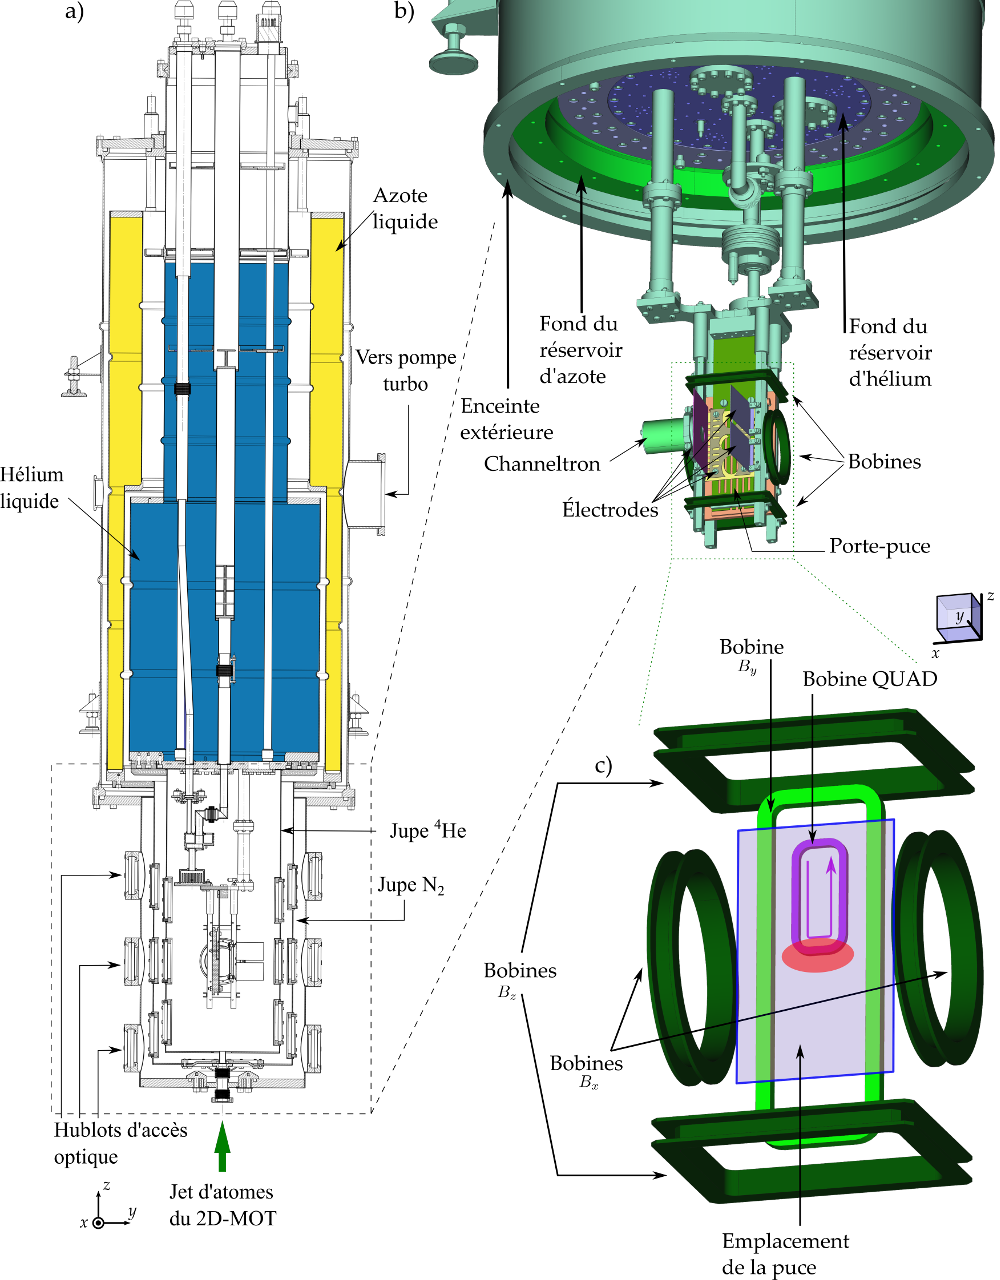
\includegraphics[width=\linewidth]{figures/cryo_vect_small.png}
\caption[Schéma du cryostat]{Schéma du dispositif cryogénique :
\textbf{a)} coupe du plan de construction du cryostat, avec la puce tournée vers le côté gauche.
Le réservoir d'azote liquide est indiqué en jaune, le réservoir d'hélium liquide en bleu.
Le c\oe ur de l'expérience est visible, ainsi que les deux \og jupes \fg{} et l'enceinte extérieure à température ambiante.
Cinq hublots, trois en face de la puce et un sur chaque côté, sont installés sur chacune de ces jupes pour l'accès optiques.
\textbf{b)} vue schématique du c\oe ur de l'expérience. La puce fait face à la direction $y$. Les bobines (vert foncé), le channeltron et les différentes électrodes sont représentées. On ne voit pas les \og jupes \fg{} d'azote et d'hélium, ni l'enceinte extérieure.
\textbf{c)} Vue de plus près des bobines : la bobine QUAD (mauve) génère un champ quadrupolaire pour faire un MOT sur puce. L'emplacement de la puce est représenté par le rectangle bleu devant la bobine QUAD et la bobine $B_y$ (vert clair).
La zone rouge indique l'endroit où les atomes de rubidium sont piégés.
}
\label{fig:cryo}
\end{figure}
%
La conception de ce cryostat a été évoquée dans la thèse de Raul Celistrino Teixeira \cite{PHD_CELISTRINO}  et discutée plus en détail dans les thèses de Thomas Nirrengarten \cite{PHD_NIRRENGARTEN} et Cédric Roux \cite{PHD_ROUX}.
Le c\oe ur de l'expérience est protégé de la radiation extérieure par des écrans thermiques (\og jupes \fg{}) en cuivre doré. Ce sont des cylindre ouverts en haut et vissés sur le fond des réservoirs de liquides cryogéniques.
La jupe $^4 \text{He}$ est vissée sur le fond du réservoir d'hélium 4 et la jupe $\text{N}_2$ est vissée au fond du réservoir d'azote liquide.
Elles sont donc respectivement thermalisées à \SIvv{4.2}{\K} et \SIvv{77}{\K}.
Sur chaque jupe, cinq hublots sont installés pour l'accès optique à la zone de piégeage :
deux sur les directions $\pm x$, un dans la direction $+y$ qui fait face à la puce, et deux  sur le plan $yz$, de part et d'autre du hublot de face sur les bissectrices des axes $+y$ et $\pm z$, appelées direction $\pm\SIvv{45}{\degree}$ respectivement.
Par ces hublots, tous les faisceaux laser atteignent la zone de piégeage au c\oe ur de l'expérience.
Tous les éléments qui sont installés à l'intérieur de la jupe hélium sont thermalisés à \SIvv{4.2}{K} par contact thermique avec le réservoir d'hélium liquide.

L'intérieur de la jupe hélium est revêtu d'une couche de plomb, supraconducteur à \Khe. Cette couche de plomb écrante les champs magnétiques extérieurs par effet Meissner \cite{MX_MEISSNEREFFECT}, et évite les courants de Foucault qui se créeraient dans les jupes à l'allumage ou à l'extinction des courants dans les bobines. 
Il reste nécessaire cependant d'imposer un champ extérieur de compensation au moment du refroidissement, afin que la couche de plomb ne piège pas de lignes de champ magnétique provenant de l'environnement.
Cette compensation du champ constant de l'environnement est réalisée à l'aide de grandes bobines placées à l'extérieur du crysotat.

Enfin, bien que les jupes ne soient pas parfaitement étanches, elles garantissent un vide différentiel entre la partie du cryostat à \SIvv{300}{\K}, où la pression vaut \SIvv{1.5e-7}{\milli\bar}, et la partie à \Khe, où la pression est inférieure à \SIvv{1e-10}{\milli\bar}\footnote{
Cette valeur n'est pas mesurée en raison de l'absence de sonde de pression dans cette région du cryostat, mais inférée à partir du temps de vie des nuages d'atomes piégés, qui est de l'ordre de la minute \cite{ENS_CHIPLIFETIME}.}.

	\subsubsection*{La puce à atomes}
\noindent La puce à atome qui siège au c\oe ur de notre expérience est représentée en figure \eqref{fig:chip}.
C'est une puce assez simple, conçue autour de trois fils supraconducteurs : le fil (LJ), en forme de \mcal{U}, le fil (LG) en forme de \mcal{Z}, et le fil (KM) droit.
Ces fils sont fabriqués par dépôt de niobium d'une épaisseur de \SIvv{2}{\um} sur un substrat de silicium recouvert d'une couche d'oxyde SiO$_2$.
Le dépôt de niobium est ensuite gravé, et l'ensemble de la puce est recouvert d'une couche d'or de \SIvv{200}{\nm} d'épaisseur afin de rendre la surface réfléchissante.
Les détails de la fabrication de la puce sont présentés en annexe dans la thèse de Raul Celistrino Teixeira \cite{PHD_CELISTRINO}.
%
\begin{figure}[]
\centering
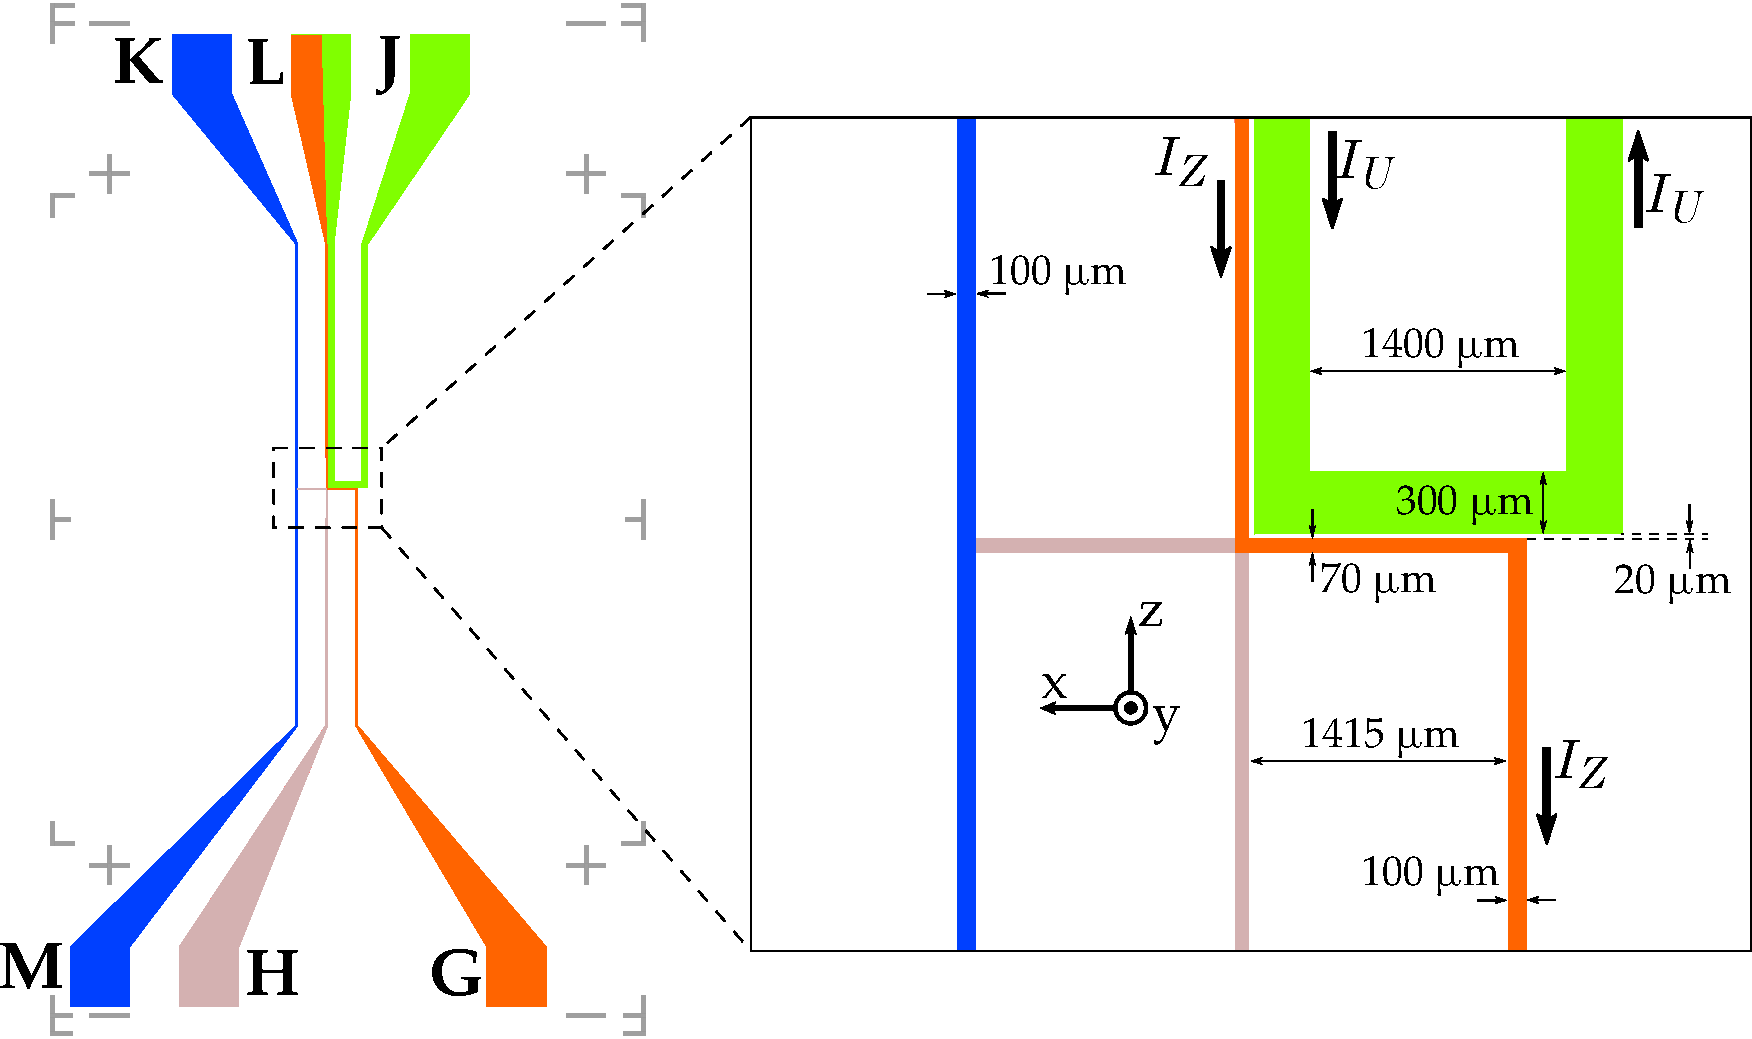
\includegraphics[width=\linewidth]{figures/chip}
\caption[Schéma de la puce à atomes supraconductrice]{Schéma de la puce supraconductrice.
Les lettres étiquettent les pattes d'entrée/sortie des courants électriques sur la puce.
Les couleurs sont une aide visuelle pour mieux suivre les fils : en vert, le \og fil \mcal{U}\fg{}, en orange le \og fil \mcal{Z}\fg{} et en bleu le \og fil RF \fg{}.
\`A droite, vue de près du centre de la puce, qui détaille la largeur des fils, la distance entre eux et le sens de circulation des courants.
Les axes $x,y$ et $z$ coïncident avec ceux de la figure \eqref{fig:cryo}.
}
\label{fig:chip}
\end{figure}
%

Les fils en \mcal{U} et en \mcal{Z} sont la simplification d'un dispositif en forme de $\mathcal{H}$ qui repose sur la circulation d'un courant perpendiculairement à deux autres courants parallèles entre eux.
La figure \eqref{fig:magfields_chip} représente les différentes configurations de champ magnétique créées par les fils \mcal{U} et \mcal{Z} de la puce.
Lors du passage d'un courant $I$ dans le fil \mcal{Z}, le segment parallèle à l'axe $x$ créé un champ qui, superposé avec un champ de biais $B_Z$ selon l'axe $z$, forme un champ quadrupolaire dans le plan $yz$.
Le courant dans les deux bras verticaux circule dans le même sens et crée un champ selon $x$, avec un  minimum non-nul au voisinage du centre du champ quadrupolaire.
Le champ total forme alors un piège magnétique de Ioffe-Pritchard (cf figure \ref{fig:magfields_chip}c)).

De façon similaire, le fil en \mcal{U} crée aussi, avec l'aide d'un champ de biais $B_Z$, un champ quadrupolaire dans le plan $yz$.
Les courants dans les bras verticaux circulent cette fois dans des sens opposés, ce qui résulte dans la présence d'un zéro de champ près du centre du champ quadrupolaire.
Le champ total permet ici la réalisation d'un piège magnéto optique sur puce en trois dimensions (\og 3D-MOT miroir\fg{}, cf figure \ref{fig:magfields_chip}d)).

\begin{figure}[]
\centering
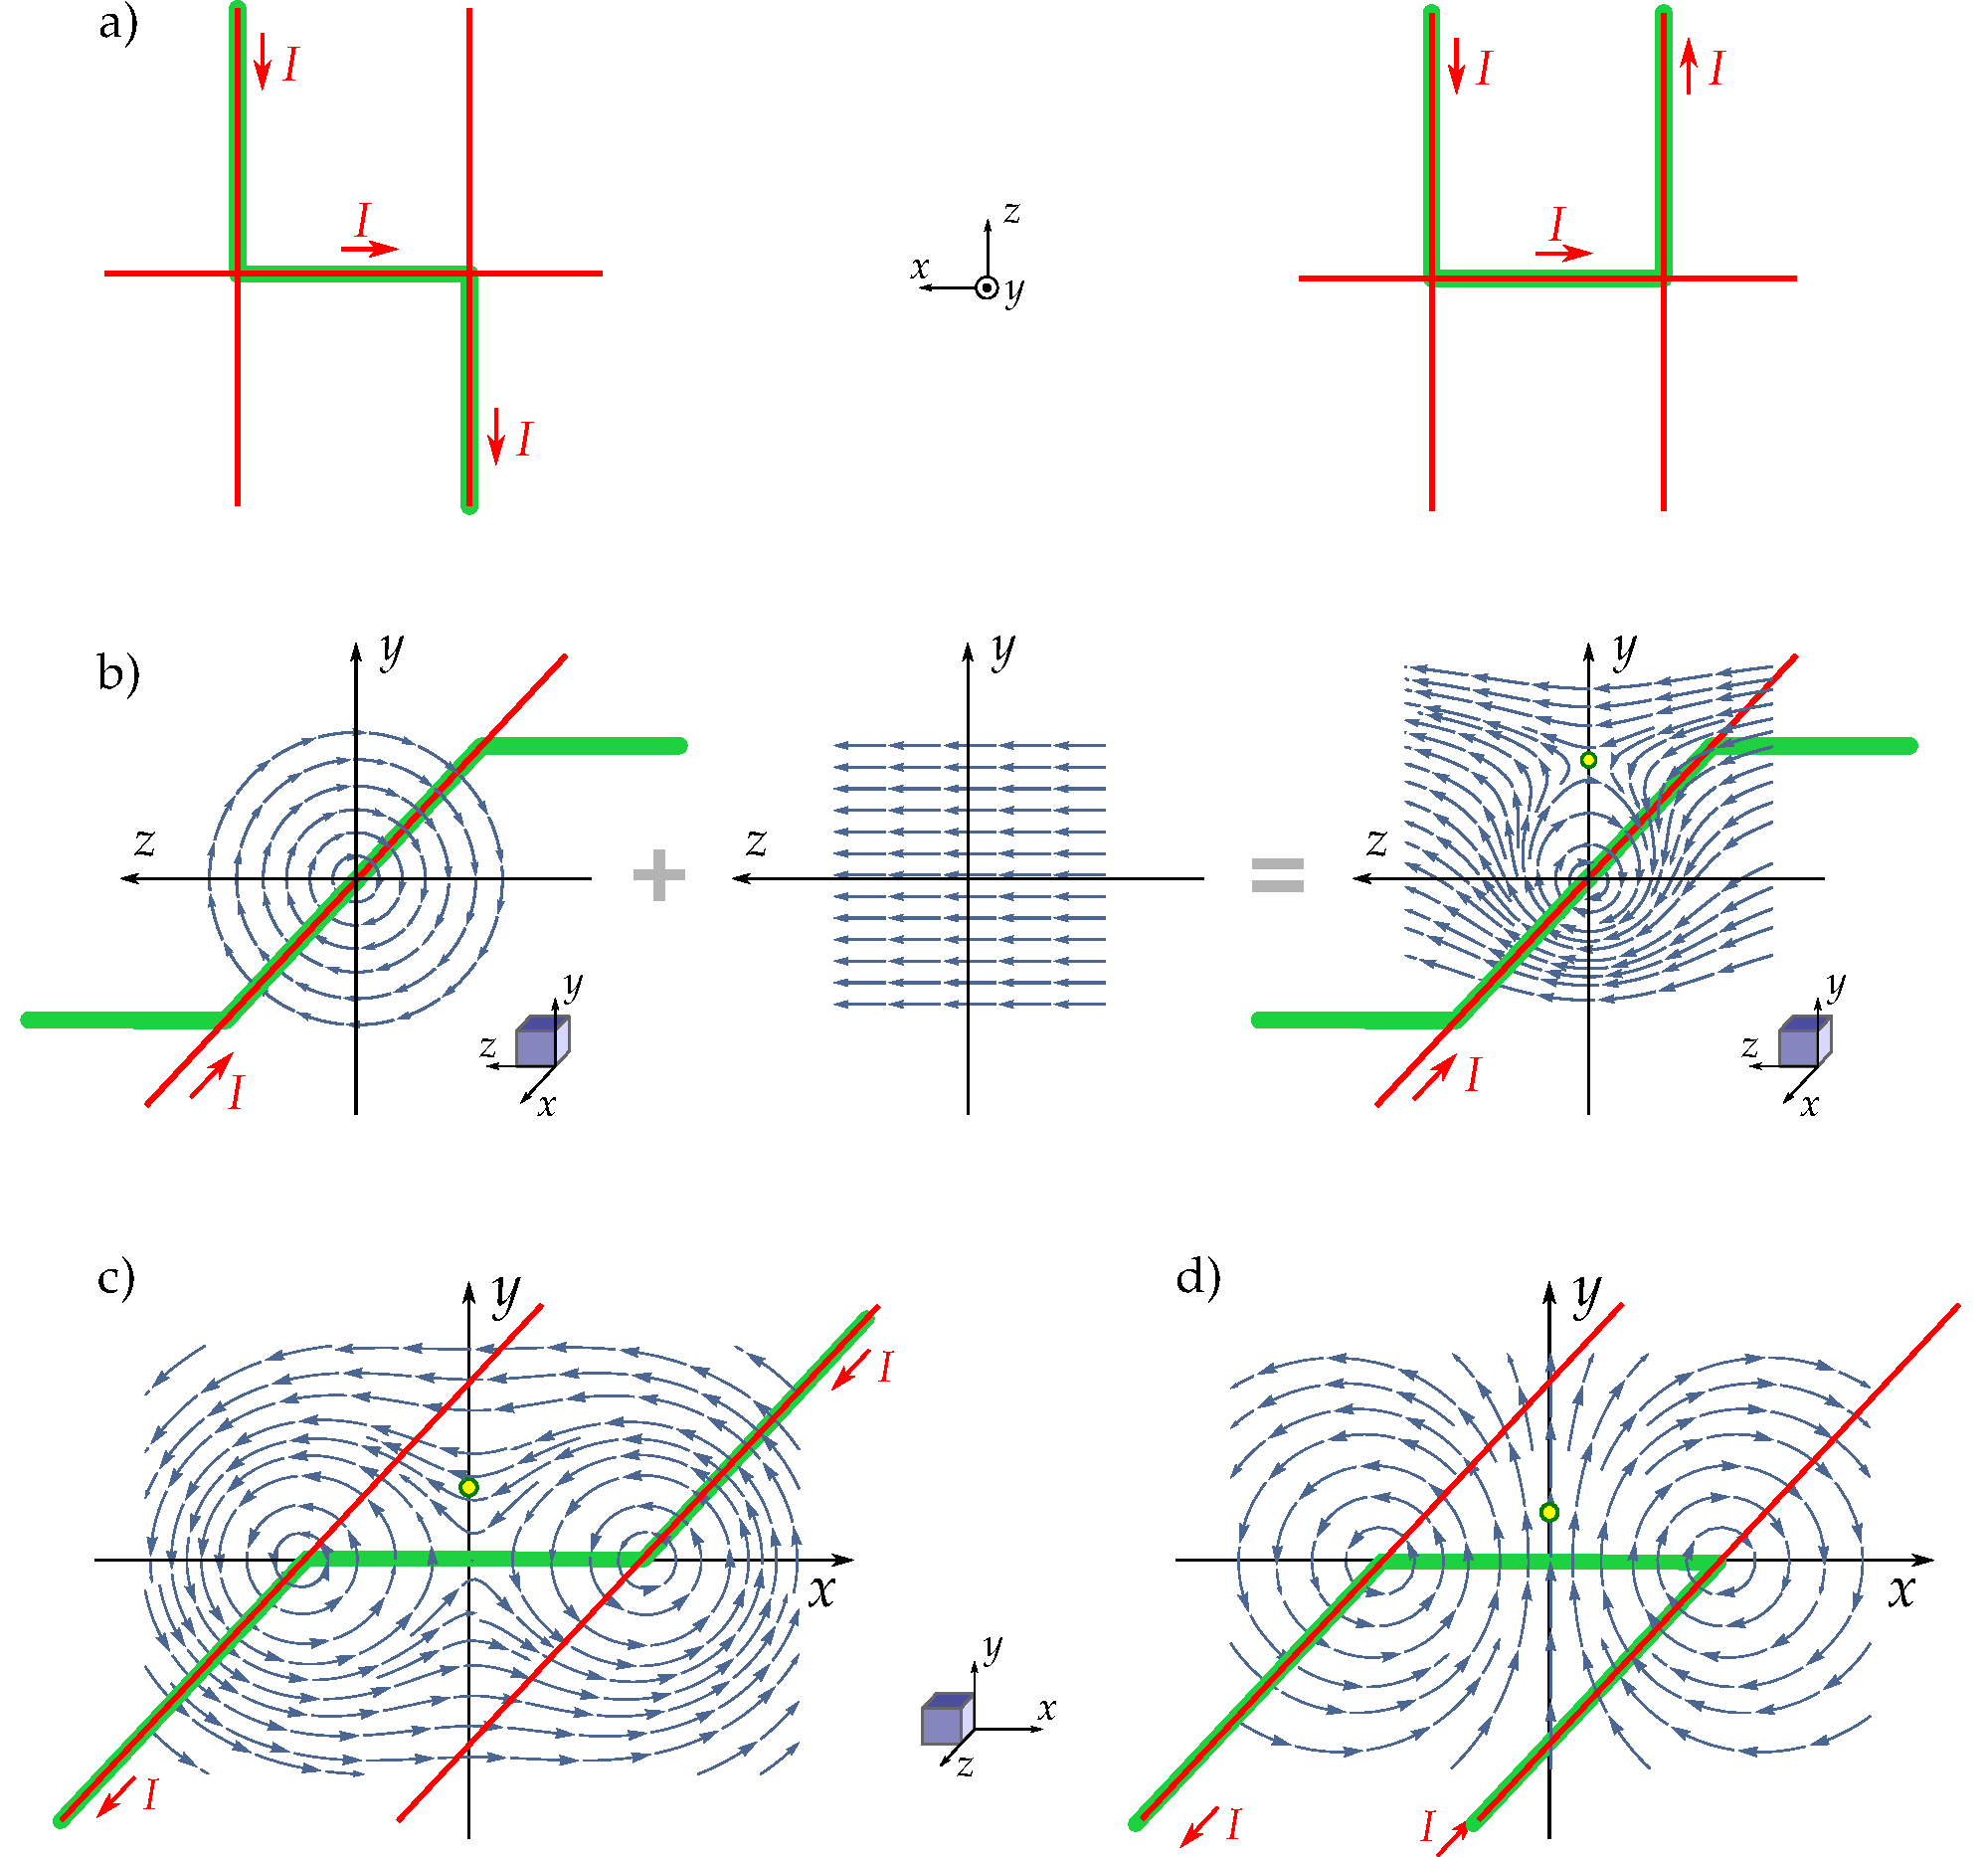
\includegraphics[width=\linewidth]{figures/magfields_chip}
\caption[Champs magnétiques créés par la puce]{
Champs magnétiques créés par la puce.
\textbf{a)} Les fils \mcal{U} et \mcal{Z} portent un courant dans la direction $x$ et une paire de courants parallèles dans la direction $z$.
\textbf{b)} Un champ quadrupolaire est créé par la superposition du courant selon $x$ et d'un champ de biais $B_Z$.
Les courants verticaux peuvent circuler soit (\textbf{c)}) dans le même sens,  soit (\textbf{d)}) dans des sens opposés.
Le module du champ total présentera alors respectivement un minimum non-nul ou nul aux positions marquées par les points jaunes.
}
\label{fig:magfields_chip}
\end{figure}

Pour le fil en \mcal{Z} comme pour le fil en \mcal{U}, le centre du piège se situe à une distance de la puce valant approximativement
\begin{equation}
\label{eq:trap_center}
r_0 \simeq \frac{\mu _0}{2\pi}\frac{I}{B_Z}
\end{equation}
et le gradient de champ magnétique à cet endroit vaut
\begin{equation}
\label{eq:trap_center_grad}
|B'(r_0)|=\frac{2\pi}{\mu _0} \frac{B_Z^2}{I} = \frac{B_Z}{r_0} = \frac{\mu _0}{2\pi}\frac{I}{r_0^2}~.
\end{equation}
%
C'est là une caractéristique importante de la géométrie des pièges : plus le centre du piège est proche de la puce, plus le piège sera confinant dans le plan $yz$.
Le piège s'allonge alors dans la direction $x$, prenant une forme de cigare de plus en plus anisotrope.

Comme nous l'avons mentionné, notre dispositif nous permet de mettre en \oe uvre des pièges magnéto-optiques en trois dimensions.
Dans beaucoup d'expériences d'atomes froids, ceux-ci sont réalisés à l'aide de trois paires de faisceaux laser contra-propageants, une dans chaque direction de l'espace.
Il nous est impossible d'envisager cette configuration, puisque l'axe $y$ est rendu inaccessible par la présence de la puce.
L'on peut cependant, avec deux paires de faisceaux laser seulement, simuler une configuration à six faisceaux, en utilisant la surface réfléchissante de la puce.
Le schéma de cette configuration, appelée \og MOT miroir \fg{}, est donné en figure \eqref{fig:mirror_MOT}.

\begin{figure}
\centering
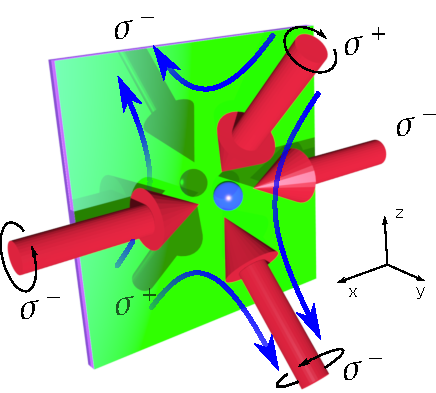
\includegraphics[width=0.6\linewidth]{figures/mirror_MOT}
\caption[Schéma de principe du MOT miroir]{Schéma de principe du MOT miroir :
Deux faisceaux contra-propageants sont envoyés parallèlement à la puce réfléchissante, selon l'axe $x$.
Les deux autres faisceaux dans le plan $yz$ viennent frapper la puce avec un angle de \SIvv{45}{\degree}.
Leur réflexion sur la puce équivaut à deux faisceaux supplémentaires d'hélicité inversée, représentés en ombre derrière la puce.
On obtient bien ainsi une configuration de MOT à six faisceaux.
}
\label{fig:mirror_MOT}
\end{figure}


	\subsection{Séquence de piégeage et refroidissement}
	
\noindent Grâce à ce dispositif, nous pouvons piéger des nuages d'atomes froids sur puce.
Nous donnons dans ce paragraphe le détail des différentes étapes de piégeage et de refroidissement des atomes.

	\subsubsection*{Système laser}
\noindent Le piégeage magnéto-optique du rubidium 87 exploite la raie D2 de celui-ci.
La raie D2 est représentée en figure \eqref{fig:D2lineRb87} avec le détail des sous-niveaux hyperfins des niveaux $\mathrm{5S_{1/2}}$ et $\mathrm{5P_{3/2}}$ du \Rb{87}.
%	
\begin{figure}
\centering
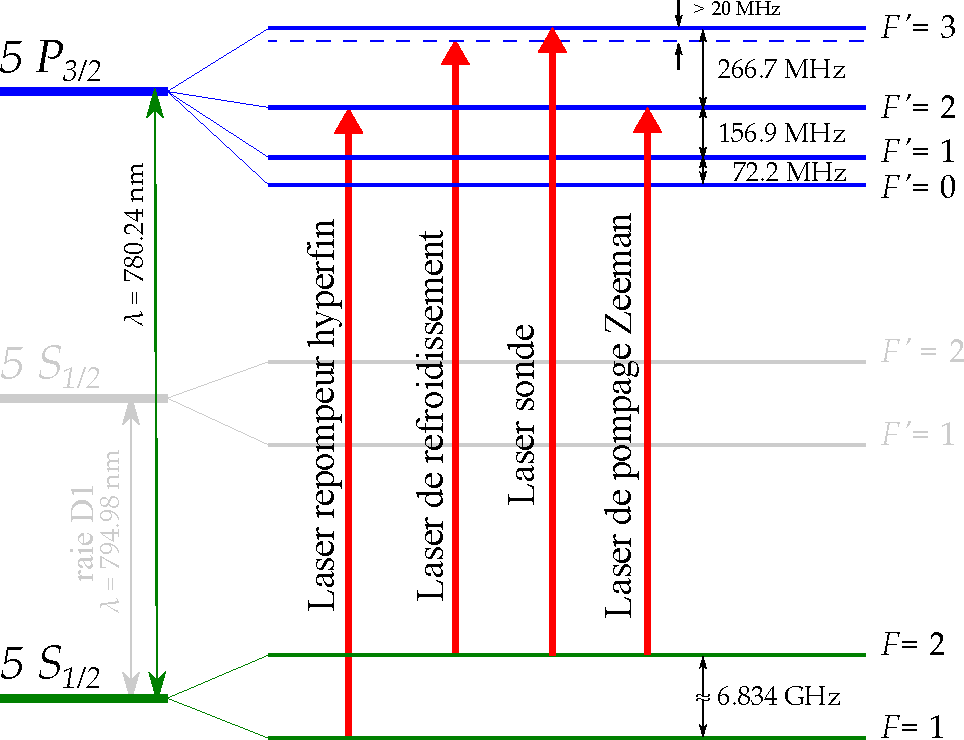
\includegraphics[width=0.8\linewidth]{figures/D2lineRb87}
\caption[Raie D2 du \Rb{87}]{Structure hyperfine de la raie D2 du \Rb{87}.
Les transitions cyclantes sont montrées pour le laser de refroidissement, le laser repompeur, le laser sonde et le laser de pompage Zeeman.
}
\label{fig:D2lineRb87}
\end{figure}
%
Nous utilisons la transition $\ket{F=2} \rightarrow \ket{F'=3}$ de la raie D2 pour piéger et refroidir les atomes.
Cette transition a une largeur naturelle $\Gamma = \SI{6.065}{\MHz}$ \cite{DATA_STECKRB87}.
Le laser de refroidissement est généré par un système commercial de diode laser amplifiée TOPTICA TA-110.
La fréquence de ce laser est asservie par battement (\og beatlock \fg{}) à un laser maître, lui-même stabilisé par une cavité Fabry-Pérot.
Cette cavité est verrouillée en fréquence sur la transition de refroidissement par absorption saturée dans une cellule de \Rb{87}.
Une commande de tension permet de définir la fréquence du battement et ainsi de contrôler rapidement le désaccord du laser de refroidissement par rapport à la transition $\ket{F=2}\rightarrow\ket{F'=3}$.

Il arrive qu'un photon du laser de refroidissement excite un atome du niveau $\ket{F=2}$ vers le niveau $\ket{F'=2}$ au lieu de $\ket{F'=3}$.
Cet atome peut alors se désexciter non pas vers le niveau $\ket{F=2}$ mais vers le niveau $\ket{F=1}$, qui est un niveau noir pour le laser de refroidissement.
Afin d'éviter le pompage des atomes vers ce niveau $\ket{F=1}$, il est nécessaire d'envoyer, avec le laser de refroidissement, un laser \og repompeur\fg{} accordé sur la transition $\ket{F=1}\rightarrow \ket{F'=2}$.
Ce laser repompeur est généré par une troisième diode laser, et indépendamment verrouillé en fréquence par absorption saturée.

Les lasers de sonde et de pompage Zeeman sont prélevés sur le laser de refroidissement et décalés en fréquence par modulation acousto-optique.
L'ensemble des faisceaux est transporté de la table optique de préparation au cryostat par des fibres optiques mono-modes à maintien de polarisation.
Ils sont enfin mis en forme à proximité immédiate du cryostat. 




	\subsubsection*{Piégeage magnéto-optique}
\noindent	Notre dispositif repose sur trois stades de piégeage magnéto-optique successifs.
Les atomes de rubidium sont stockées dans une cellule en verre, ouverte vers une enceinte sous ultra-vide (UHV) située à l'extérieur du cryostat.
Dans cette enceinte, les atomes sont piégés le long de l'axe $z$ par un piège magnéto-optique en deux dimensions (\og 2D-MOT \fg{}).
Celui-ci est schématisé en figure \eqref{fig:2DMOT}.
%	
\begin{figure}
\centering
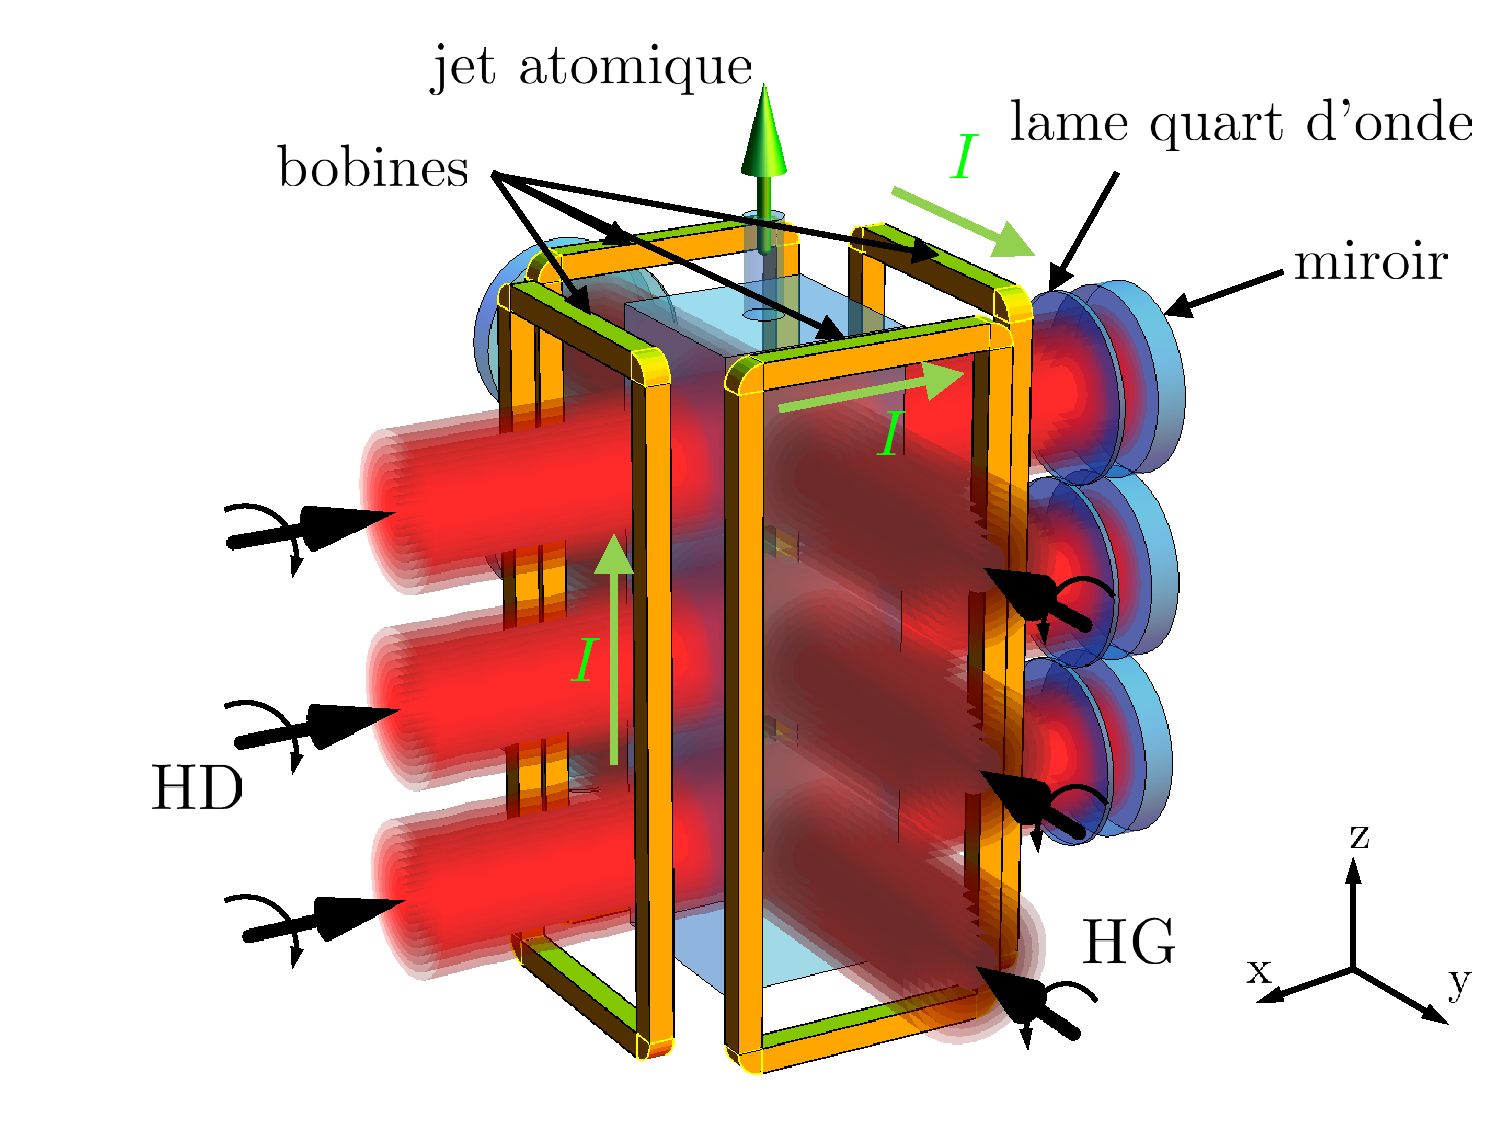
\includegraphics[width=0.6\linewidth]{figures/2DMOT}
\caption[Schéma du 2D-MOT]{Schéma du 2D-MOT avec ses trois étages de piégeage.
Les polarisations des faisceaux incidents sont indiquées par les lettres HD (pour hélicité droite) et HG (hélicité gauche), relativement à la direction de propagation des faisceaux.
Le sens des courants dans les bobines est indiqué par les flèches verts et la lettre $I$.
Chaque faisceau est rétro-réfléchi par un miroir, et le double passage par une lame quart d'onde permet de garantir la bonne polarisation du faisceau réfléchi.
Le jet atomique produit par le 2D-MOT est représenté par une flèche qui pointe vers le cryostat.
}
\label{fig:2DMOT}
\end{figure}
%
L'ensemble du 2D-MOT a été conçu et fabriqué par la laboratoire SYRTE de l'Observatoire de Paris.

Les atomes piégés dans le 2D-MOT diffusent librement selon l'axe $z$, formant un jet vertical qui arrive jusqu'à la puce atomique à l'intérieur du cryostat.
Les atomes sont alors capturés dans un MOT de grand volume créé par les bobines de biais et le bas de la bobine \og QUAD \fg{}, représentée en figure \eqref{fig:cryo}.
Le bas de la bobine QUAD permet de créer un champ quadrupolaire similaire à celui du fil \mcal{U}, adapté au piégeage magnéto-optique.
Le nombre de spires $n=19$ de la bobine permet de multiplier par autant le courant générateur de champ dans l'équation \eqref{eq:trap_center}.
Le grand volume du champ quadrupolaire ainsi créé permet de capturer efficacement les atomes du jet.
Le chargement de ce gros \og QAUD-MOT \fg{} dure de \SIvv{1}{} à \SIvv{3}{\s}, pendant lesquels on peut y collecter quelques \SIvv{e8} atomes à une température de l'ordre de \SIvv{400}{\uK}.

Le nuage atomique est alors transféré vers un second MOT, créé cette fois par les bobines de biais et le fil \mcal{U}, comme nous l'avons mentionné en \ref{subsec:cryopuce}.
Ce \og U-MOT lointain\fg{} présente des gradients similaires au QUAD-MOT mais un volume plus petit.
Le taux de transfert entre les deux est estimé entre $\num{10}$ et $\SI{40}{\percent}$ par des observations en fluorescence du nuage.
Nous pouvons à ce moment réduire le courant dans le fil \mcal{U}, ce qui d'après les équations \eqref{eq:trap_center} et \eqref{eq:trap_center_grad} rapproche le piège de la surface de la puce et le comprime en augmentant le gradient de champ.
Les gradients de champs étant plus forts, la force de rappel de la lumière s'en trouve grandie.
On peut alors se permettre d'augmenter le désaccord des faisceaux lasers afin de refroidir le nuage atomique.
Les températures atteintes dans ce \og U-MOT proche\fg{} sont de l'ordre de $\SI{40}{\uK}$, pour un nuage d'environ $\numrange{e7}{e8}$ atomes.

	\subsubsection*{Les étapes intermédiaires : mélasse optique et pompage Zeeman}
\noindent L'objectif, après les étapes de piégeage magnéto-optique, est de transférer les atomes dans le piège de Ioffe-Pritchard créé par le fil \mcal{Z}.
Cela sera d'autant plus efficace que le nuage atomique sera froid, et que les atomes seront bien polarisés dans le sous-niveau Zeeman $m_F=+2$ du niveau hyperfin $\mathrm{5S1/2,F=2}$.
Avant de les transférer vers le \og piège Z \fg{}, nous faisons donc subir aux atomes deux phases supplémentaires.

Tout d'abord, nous éteignons les champs magnétiques du U-MOT en laissant les faisceaux lasers allumés.
Cela initie une étape de mélasse optique d'une durée comprise entre $\num{1} et \SI{5}{\ms}$, au cours de laquelle le désaccord laser est augmenté alors que la puissance lumineuse est graduellement diminuée jusqu'à zéro.
Cette mélasse optique nous permet de refroidir quelques $\numrange{e6}{e7}$ atomes à des températures inférieures à $\SIvv{10}{\uK}$.

Après l'extinction des lasers de mélasse, un champ magnétique de \SIrange{1}{2}{\gauss} est rapidement allumé sur la direction $-y$, qui lève la dégénérescence des sous-niveaux Zeeman.
Un laser de pompage optique polarisé $\sigma ^+$ se propageant selon $-y$ pompe alors les atomes dans le sous-niveau $m_F=+2$.
Après réflexion sur la puce ce faisceau laser repasse à travers le nuage atomique.
Son hélicité a certes été inversée par la réflexion, mais sa polarisation du point de vue des atomes est restée la même.
Les atomes sont donc encore pompés vers le sous-niveau $m_F=+2$.

	\subsubsection*{Le piégeage magnétique et le refroidissement évaporatif}
\noindent Lorsque le nuage atomique est bien refroidi et polarisé par les étapes de mélasse et de pompage optique, le piège magnétique est allumé.
Pour cela, un courant est imposé dans le fil \mcal{Z}.
Un champ $B_z$ est généré par les bobines, qui permet d'obtenir un champ quadrupolaire comme nous l'avons évoqué en \ref{subsec:cryopuce}, centré sur la position du nuage atomique.
Le champ au centre du piège est alors orienté selon la direction $x$ et le minimum de champ, strictement supérieur à $0$, permet d'éviter les pertes de Majorana par retournement du spin.
Un second champ de biais, $B_x$, permet en outre de limiter les pertes atomiques dues à la présence d'un bruit radio-fréquence dans notre expérience.
Ce bruit peut en effet causer des transitions atomiques vers les états non piégés $m_F<1$ et il s'agit d'ajuster $B_x$ afin d'éviter que les transitions ne soient résonantes avec la fréquence du bruit \cite{PHD_NIRRENGARTEN}.

Une fois allumé, le piège magnétique est immédiatement comprimé afin d'augmenter le taux de collision entre les atomes en vue du refroidissement évaporatif.
La compression du piège est réalisée adiabatiquement en \SI{150}{\ms}.
Le piège comprimé a des fréquences de piégeage de l'ordre de $(\omega_x,\omega_y,\omega_z) \simeq 2\pi \times (\num{24},\num{3400},\num{3400})\si{\hertz}$ à une distance de \SI{80}{\um} de la puce.
Nous pouvons alors mettre en \oe uvre une séquence de refroidissement évaporatif radio-fréquence :
les atomes les plus chauds sont transférés vers les sous-niveaux Zeeman non piégés par des transitions radio-fréquence (RF), et ainsi sont éjectés du piège.
La fréquence de ces transitions dépend du champ magnétique vu par chaque atome, et donc de sa position dans le potentiel de piégeage.
La fréquence du signal RF, envoyé dans le fil vertical (KM) de la puce (cf figure \ref{fig:chip}), est progressivement diminuée afin d'évaporer les atomes les plus chauds en premier, puis de plus en plus froids.
Le reste du nuage thermalise vite grâce au taux de collision élevé et se trouve ainsi refroidi.
Plusieurs rampes de fréquence successives sont optimisées en durée et en puissance RF, afin d'obtenir le meilleur refroidissement du nuage atomique.
L'étape de refroidissement évaporatif dure de \SIrange{0}{5}{\second} au total.
Le schéma de principe du refroidissement évaporatif RF est donné en figure \eqref{fig:evapRF}.
%
\begin{figure}[]
\centering
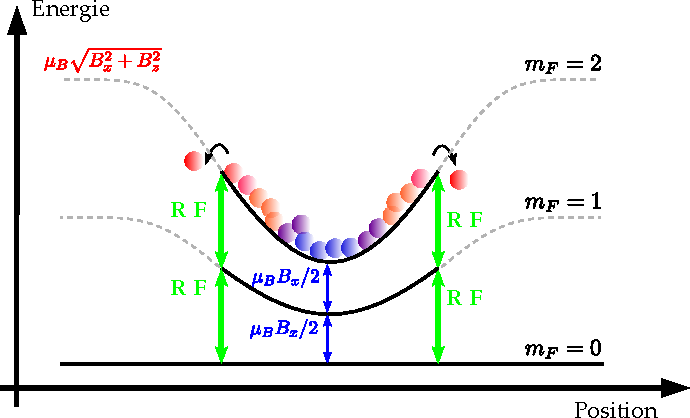
\includegraphics[width=.7\linewidth]{figures/evapRF}
\caption[Refroidissement évaporatif RF]{Refroidissement évaporatif radio-fréquence :
le \og couteau \fg{} RF induit les transitions entre sous-niveaux Zeeman.
Une fois dans les sous-niveaux $m_F<1$, les atomes ne sont plus piégés et sont éjectés du piège.
L'aile chaude de la distribution de Boltzmann est évacuée et les atomes restant sont thermalisés à une température plus faible.
}
\label{fig:evapRF}
\end{figure}

Cette étape de refroidissement nous permet d'abaisser la température du nuage sous le seuil de condensation de Bose-Einstein.
Nous pouvons ainsi produire de façon reproductible des condensats sur puce contenant de \SIrange{10000}{20000}{} atomes.
La séquence de refroidissement peut également être interrompue avant la condensation, et en choisissant la fréquence finale de la rampe RF, nous pouvons choisir la température du nuage atomique.
La figure \eqref{fig:BEC} montre des images du nuage atomique après temps de vol pour différentes valeurs de la fréquence finale de la rampe RF.
%
\begin{figure}[]
\centering
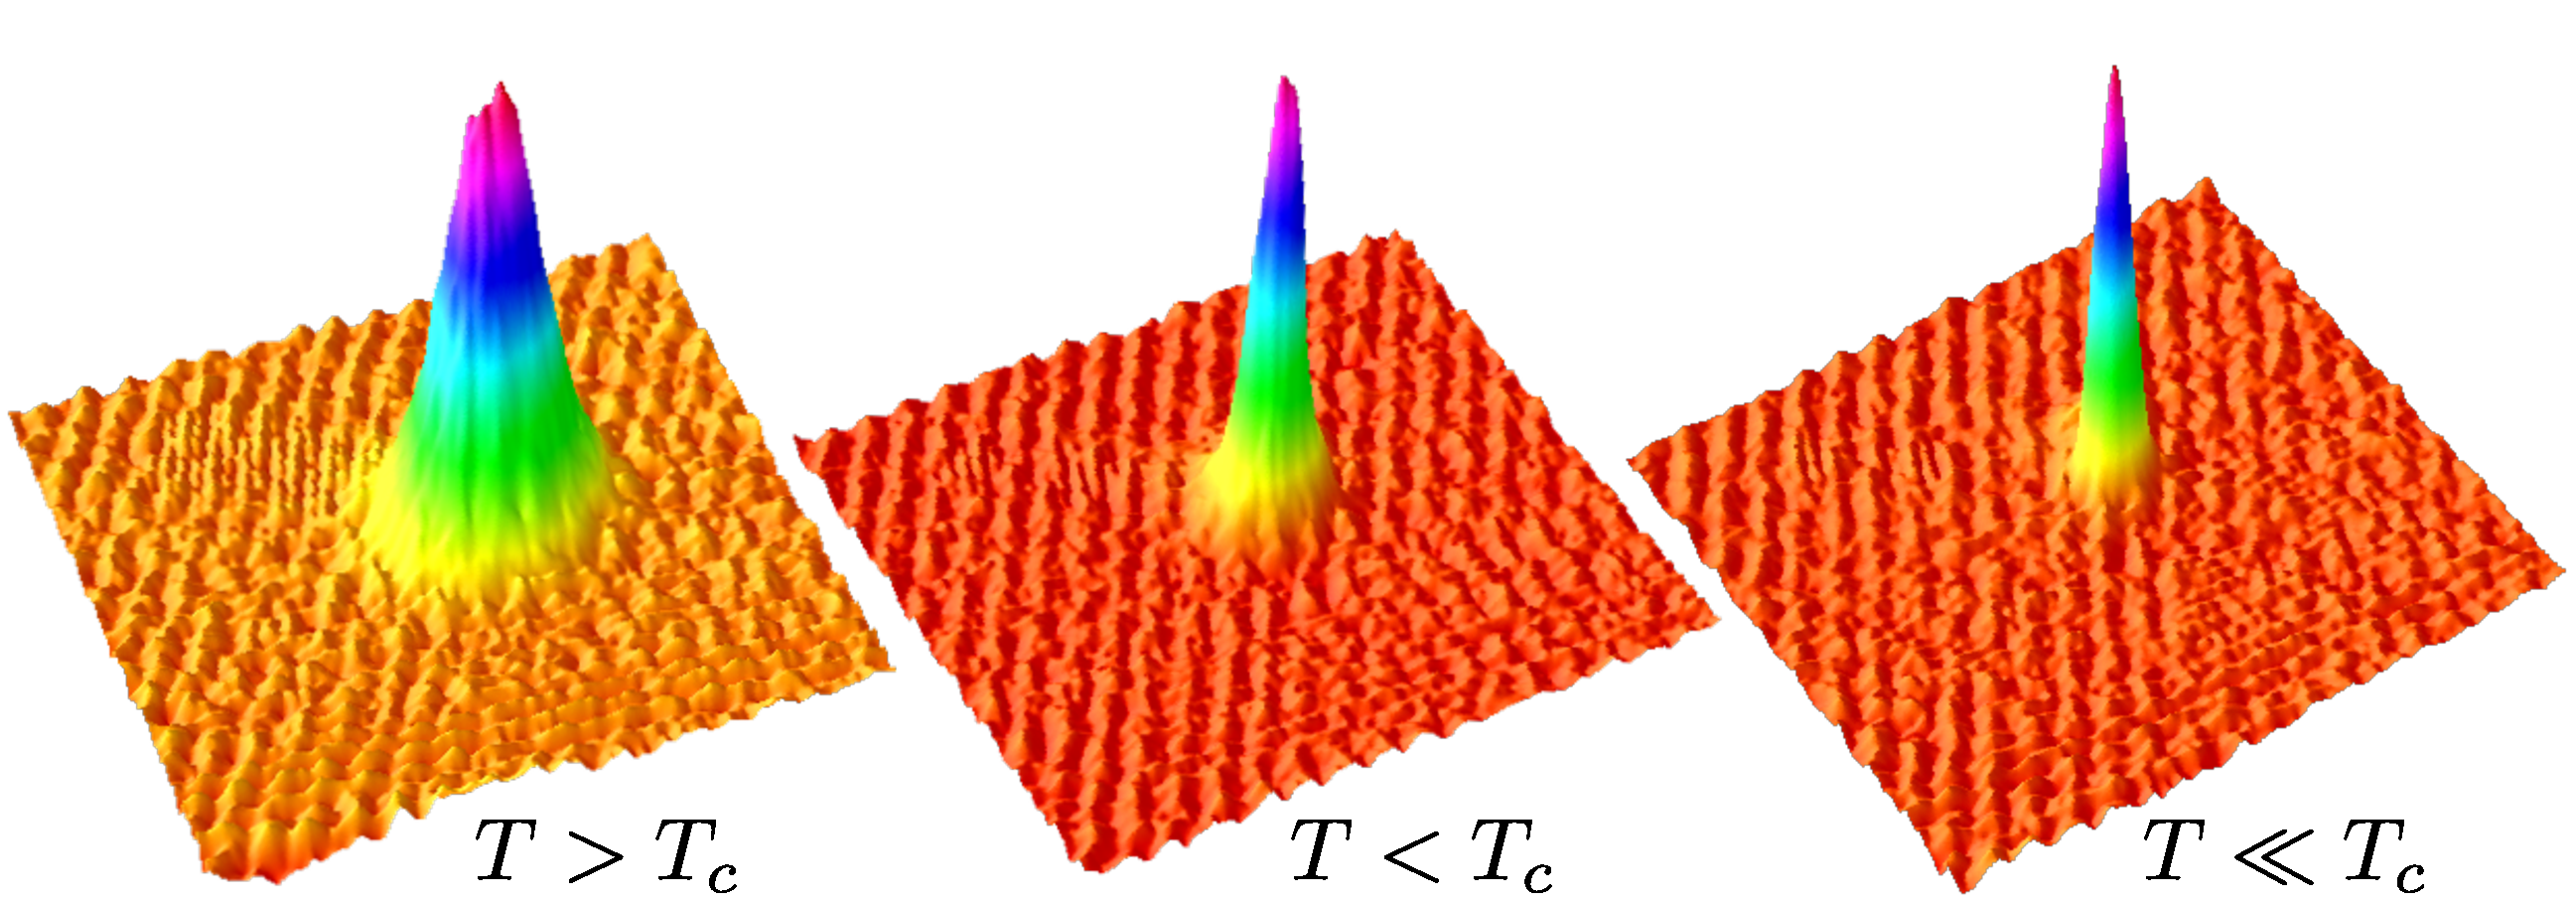
\includegraphics[width=1\linewidth]{figures/BEC}
\caption[Condensat de Bose-Einstein sur puce]{
Trois nuages de \Rb{87} évaporés jusqu'à des valeurs différentes de fréquence RF, imagés après un temps de vol de \SI{16.5}{\ms}.
Les images donnent directement la distribution d'impulsion au sein du nuage.
\`A gauche, la température est supérieure à la température critique de condensation $T_C$: le nuage est purement thermique et montre une distribution gaussienne d'impulsion.
Au milieu, la température est inférieure à $T_C$, le nuage montre un double profil en impulsion : un condensat de Bose-Einstein au centre et les atomes du nuage thermique autour.
\`A droite, la température est très petite devant $T_C$ et le condensat est quasi-pur : le nuage présente un profil de Thomas-Fermi dans l'espace des impulsions.
}
\label{fig:BEC}
\end{figure}
%

Enfin, une fois le nuage refroidi à la température souhaitée, le piège magnétique est décomprimé.
Cela permet de choisir soit une distance particulière du nuage atomique à la puce, soit la taille du nuage atomique final.

Les atomes qui seraient restés dans le sous-niveau $m_F=+1$ peuvent à leur tour être éliminés du piège en envoyant sur le nuage un signal micro-onde à \SI{6.8}{\GHz} adressant la transition hyperfine $\ket{F=2,m_F=1} \rightarrow \ket{F=1,m_F=0}$.
En présence d'un champ magnétique, les sous-niveaux Zeeman sont suffisamment résolus pour adresser uniquement cette transition, sans affecter les atomes dans le niveau $\ket{F=2,m_F=+2}$.

Une séquence expérimentale typique est présentée en figure \eqref{fig:exp_sequence}.
Cette figure détaille les paramètres expérimentaux à chaque étape du piégeage et du refroidissement des atomes.
L'étape d'élimination des atomes restant en $m_F=+1$ n'est pas représentée.
Les étapes d'excitation et détection Rydberg et d'imagerie atomique seront discutées dans la suite de ce chapitre.

%	
\begin{sidewaysfigure}
\centering
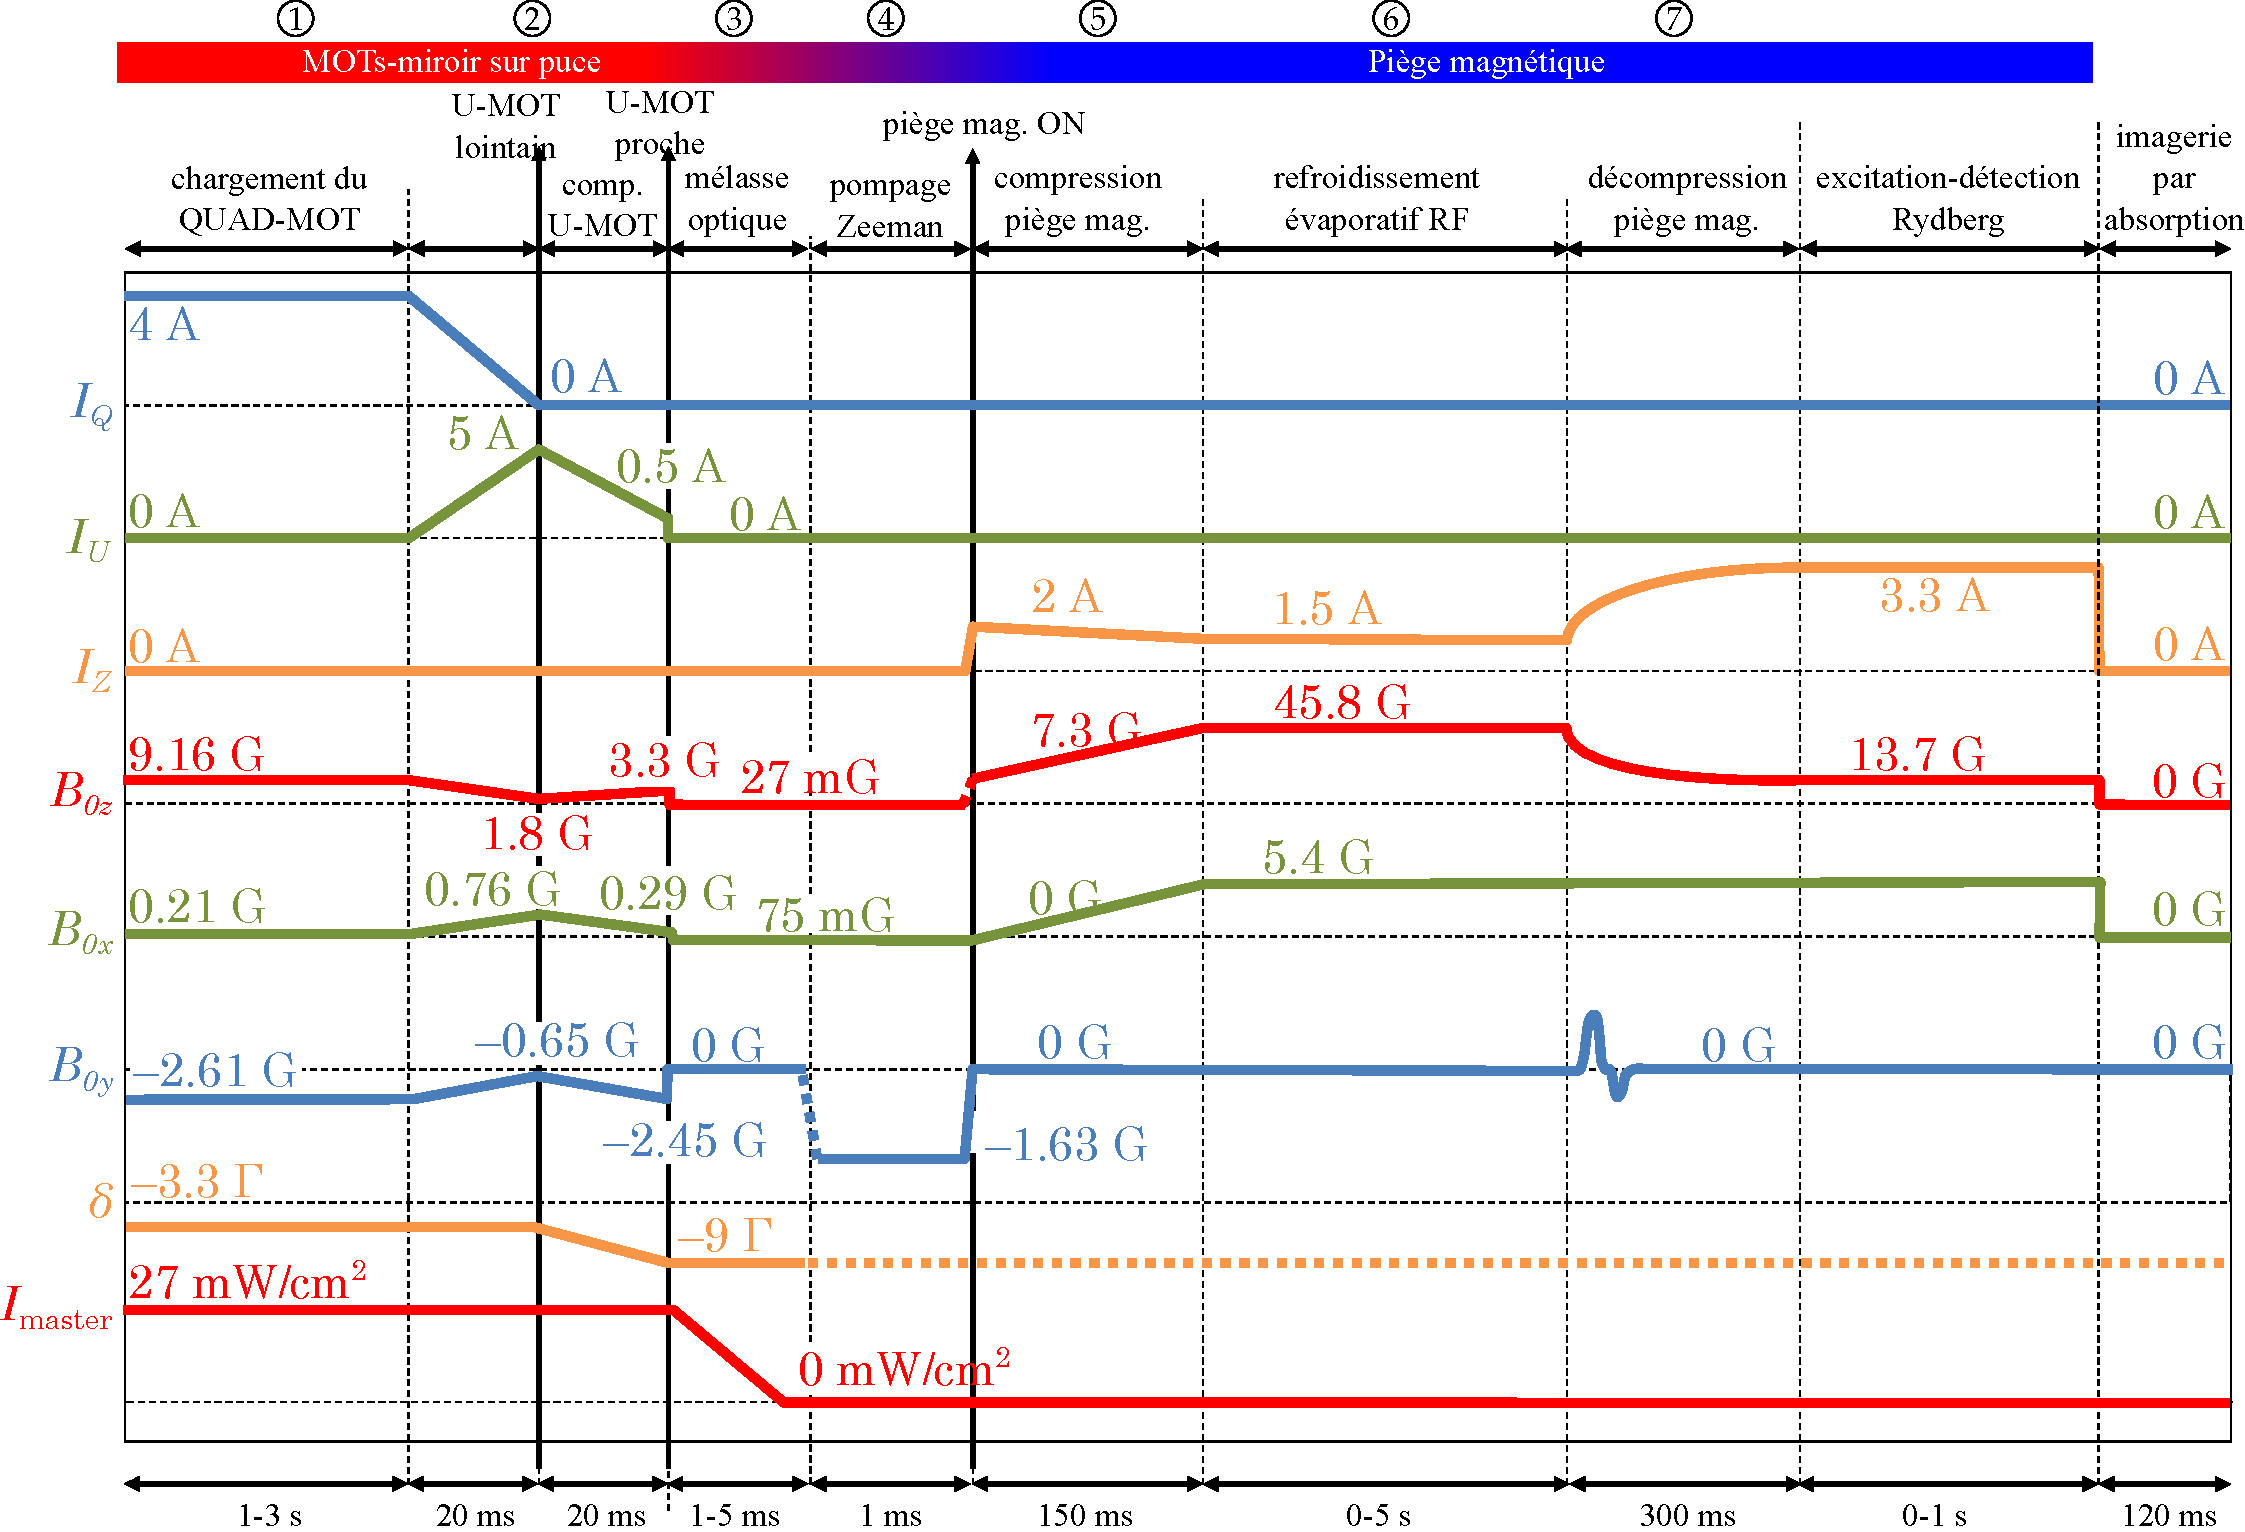
\includegraphics[width=\linewidth]{figures/exp_sequence}
\caption[Séquence expérimentale typique]{Séquence expérimentale typique : la durée et les valeurs des paramètres à chaque étape sont précautionneusement optimisés.
Les étapes de piégeage et de refroidissement sont numérotées de \numrange{1}{7} et discutées dans le texte.
Les étapes ultérieures seront décrites par la suite.
$I_{Q,U,Z}$ sont les courants dans la bobine QUAD, le fil \mcal{U} et le fil \mcal{Z}, en Ampères.
$B_{0~x,y,z}$ sont les champs de biais générés par les bobines dans les directions $x,y,z$, en Gauss.
$\delta$ est le désaccord du laser en unité de la largeur de raie $\Gamma=\SI{6.065}{\MHz}$, et $I_{master}$ son intensité en \si[per-mode=symbol]{\milli\watt \per\squared\cm}.
}
\label{fig:exp_sequence}
\end{sidewaysfigure}

		
	\subsection{Imagerie atomique par absorption}
	
\noindent Dans une expérience d'atomes froids, il est essentiel de pouvoir imager et dénombrer correctement le nuage atomique.
L'imagerie par absorption est une technique précise et efficace pour cela.
%Elle consiste à envoyer sur les atomes un faisceau laser, résonnant avec une transition atomique choisie, et à mesurer quelle fraction de la lumière le nuage atomique a absorbé.
Lorsqu'une telle expérience est menée au c\oe ur d'un cryostat, la tâche est rendue plus difficile en raisons des accès optiques limités qui contraignent fortement l'optique d'imagerie.

	\subsubsection*{Dispositif optique}

Nous pouvons imager notre nuage atomique de deux façons différentes.
Un premier faisceau sonde (\og sonde face \fg{})  entre dans le cryostat et en ressort perpendiculairement à la puce après réflexion sur celle-ci, par le hublot de face.
Un miroir percé permet de laisser passer le faisceau d'entrée et de collecter le faisceau de sortie, qui est ensuite envoyé vers une caméra CCD.
Grâce à l'installation d'une lentille de courte focale à la place du hublot de face sur la jupe hélium du cryostat, cet axe d'imagerie peut collecter beaucoup de lumière, avec une limite de résolution intéressante.

Un deuxième faisceau sonde (\og sonde côté \fg{}) est envoyé par un hublot de côté ($+x$), se réfléchit sur la puce avec un angle variant de \SIrange{5}{10}{\degree}, et ressort par l'autre hublot de côté ($-x$). Il est ensuite envoyé vers une autre caméra CCD.
Cet axe d'imagerie ne dispose pas d'une lentille interne au cryostat. Ainsi, la lumière collectée et la résolution optique sont limitées par le diamètre de la première lentille après la sortie du cryostat.
Cette lentille est donc placée le plus près possible de l'enceinte du cryostat.
En raison de cette géométrie, l'imagerie des atomes par la sonde côté forme deux images du nuage atomique : celui absorbe à la fois le faisceau incident et le faisceau réfléchi sur la puce.
Cela nous permet d'évaluer précisément la distance du nuage atomique à la puce : elle vaut la moitié de la distance entre les deux images du même nuage.
La figure \eqref{fig:double_cloud} montre une image d'absorption de la sonde côté par un nuage froid (piégé magnétiquement et refroidi), après un temps de vol de \SI{16.5}{\ms}.
Le dispositif optique d'imagerie est représenté en figure \eqref{fig:probes_CdF}.
%	
\begin{figure}
\centering
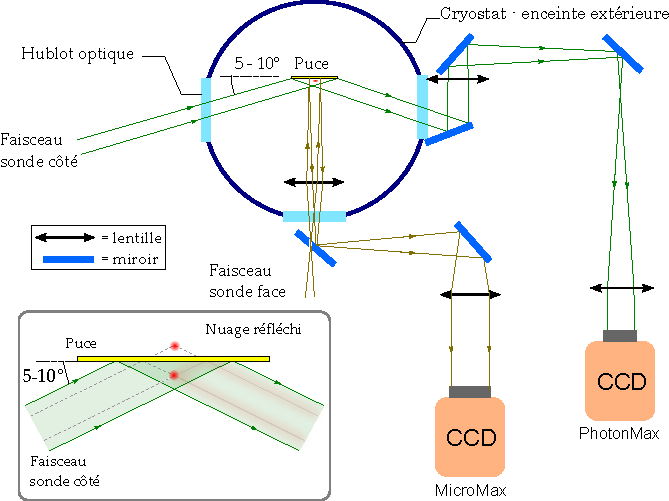
\includegraphics[width=.7\linewidth]{figures/probes_CdF}
\caption[Faisceaux sonde]{Schéma optique des faisceaux sonde dans le cryostat.
L'insert montre de plus près la réflexion du faisceau sonde côté sur la puce et la formation des deux images du nuage.
}
\label{fig:probes_CdF}
\end{figure}

%	
\begin{figure}
\centering
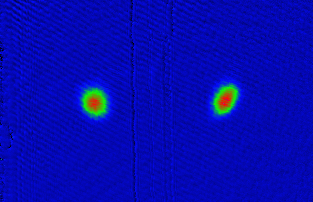
\includegraphics[width=.6\linewidth]{figures/double_cloud}
\caption[Image par absorption du nuage par la sonde côté]{Image par absorption d'un nuage froid après temps de vol, éclairé par la sonde de côté. Les deux images du nuage sont dues à la réflexion du faisceau sur la puce.
On distingue, entre les deux images du nuage atomique, les ombres portées par les fils de la puce.
}
\label{fig:double_cloud}
\end{figure}

	\subsubsection*{Principe de l'imagerie par absorption}
	
Les atomes peuvent être observés en temps réel par la collecte des photons qu'ils émettent par fluorescence, mais l'imagerie par absorption permet une meilleure précision sur l'estimation du nombre d'atome dans le nuage.
Elle consiste à envoyer sur les atomes un faisceau laser, résonnant avec une transition atomique choisie, et à mesurer quelle fraction de la lumière le nuage atomique a absorbé.

Lorsque l'intensité lumineuse reçue par les atomes est largement inférieure à l'intensité de saturation, l'absorption de celle-ci est bien décrite par la loi de Beer-Lambert :
\begin{equation}
\label{eq:Beer-Lambert}
\frac{dI(x,y,z)}{dx} = -\sigma n(x,y,z) I(x,y,z),
\end{equation}
où $I(x,y,z)$ est l'intensité lumineuse au point de coordonnées $(x,y,z)$, $n$ la densité atomique en ce point, $x$ la direction de propagation du faisceau lumineux et $\sigma$ la section efficace de diffusion de la lumière par un atome unique.
L'optique d'imagerie nous oblige cependant à intégrer cette équation dans la direction de propagation $x$.
On obtient alors 
\begin{equation}
\label{eq:Beer-Lambert_integ}
I_f(y,z) = I_i (y,z). e^{-\int dx~\sigma~n(x,y,z)}
\end{equation}
où $I_i$ est l'intensité du faisceau incident et $I_f$ l'intensité du faisceau à la sortie du nuage atomique.

Les images enregistrées par les caméras permettent d'obtenir les quantités $I_i(y,z)$ et $I_f(y,z)$.
On peut alors calculer la densité optique du nuage , définie comme $OD(y,z) = \int dx~\sigma~n(x,y,z)$, et qui d'après l'équation \eqref{eq:Beer-Lambert_integ} est égale à
\begin{equation}
\label{eq:OD}
OD(y,z) = \int dx~\sigma~n(x,y,z) = -\ln \frac{I_f(y,z)}{I_i(y,z)}.
\end{equation}
L'on en extrait ensuite la densité atomique intégrée le long de l'axe de propagation du laser à partir de l'équation \eqref{eq:OD} :
\begin{equation}
\label{eq:atomic_density}
n(x,y) = \int{dx~n(x,y,z)} = -\frac{1}{\sigma} \ln \frac{I_f(x,y)}{I_i(x,y)} = \frac{OD(y,z)}{\sigma}.
\end{equation}
		
Dans le cas simple d'une lumière résonante avec  une transition non-dégénérée, la section efficace de diffusion $\sigma$ est donnée directement par la section efficace de diffusion résonante 
\begin{equation}
\sigma = \sigma_0 = \frac{3\lambda^2}{2\pi},
\end{equation}
où $\lambda$ est la longueur d'onde de la lumière résonante.
Les atomes dans notre piège magnétique sont préparés dans l'état $\ket{5S1/2,F=2,m_F=+2}$, et la lumière de sonde est préparée de façon à adresser la transition $\sigma^+$ vers le niveau $\ket{5P3/2,F=3,m_F=+3}$.

\subsubsection*{Corrections et améliorations de l'imagerie par absorption}
\noindent Malgré l'apparente simplicité du dispositif d'imagerie par absorption, plusieurs effets perturbent les mesures du nombre d'atomes et méritent d'être corrigés.

Premièrement, la section efficace de diffusion $\sigma$ dans notre expérience n'est pas égale à la section efficace de diffusion résonante $\sigma_0$.
En effet, la lumière des faisceaux sonde n'est pas parfaitement polarisée $\sigma^+$.
De plus, les atomes ne sont pas tous dans le sous-niveau $m_F=+2$, en particulier lorsque l'on souhaite imager le nuage dans le MOT ou après l'étape de mélasse optique sans le charger dans le piège magnétique.
Enfin, l'interférence entre le faisceau sonde de côté et sa réflexion sur la puce module l'intensité de la lumière vue par le nuage atomique.
La combinaison de ces effets réduit la section efficace de diffusion d'un facteur $\alpha$, que l'on sait calibrer expérimentalement \cite{PHD_CELISTRINO,MX_GUERYODELIN_SATABSIM}.
Pour l'absorption de la sonde de côté par un nuage dans le piège magnétique, nous obtenons une valeur $\alpha_{magn} = \num{2.06} \pm \num{0.1}$.
Pour l'absorption de la sonde de côté par un nuage juste après la mélasse optique, nous obtenons une valeur $\alpha_{melasse} = \SI{2.27}{} \pm \SI{0.1}{}??????????????????????????$.
Le nombre d'atomes évalué à partir des images par absorption dépend directement de la valeur de ce paramètre $\alpha$.
	
Deuxièmement, l'acquisition du signal d'imagerie se fait en trois temps.
Une première image est enregistrée où les atomes absorbent le faisceau sonde, ce qui nous donne l'intensité $I_f$.
Puis une deuxième image est enregistrée après que les atomes sont tombés par gravité, qui nous donne l'intensité du faisceau sonde non absorbé $I_i$.
Enfin, une troisième image est enregistrée, qui permet de soustraire la lumière de fond et le bruit électronique des deux images précédentes.
Les délais de quelques dizaines de \si{\ms} entre les différentes images ont un effet délétère sur le signal : des vibrations et déformations lentes de la structure qui tient le cryostat et des variations d'indice de l'air le long du chemin optique génèrent des franges dans les images traitées par l'équation \eqref{eq:atomic_density}, semblables à des franges d'interférence.
Ce problème se présente principalement sur l'imagerie par la sonde de face en raison des plus grands délais exigés par la caméra.
Afin d'y remédier, nous avons implémenté un algorithme de réduction des franges qui, à partir d'une base de plusieurs images du faisceau sonde seul, reconstitue la meilleure combinaison linéaire de celles-ci pour chaque image où le nuage atomique est présent. Cet algorithme est décrit en détail dans \cite{MX_WHITLOCK_FRINGEREDUCTION}.
La figure \eqref{fig:Fringe_Reduction} montre une image d'un nuage froid par absorption de la sonde face, non traitée et après traitement par cet algorithme.

\begin{figure}[!h]
\centering
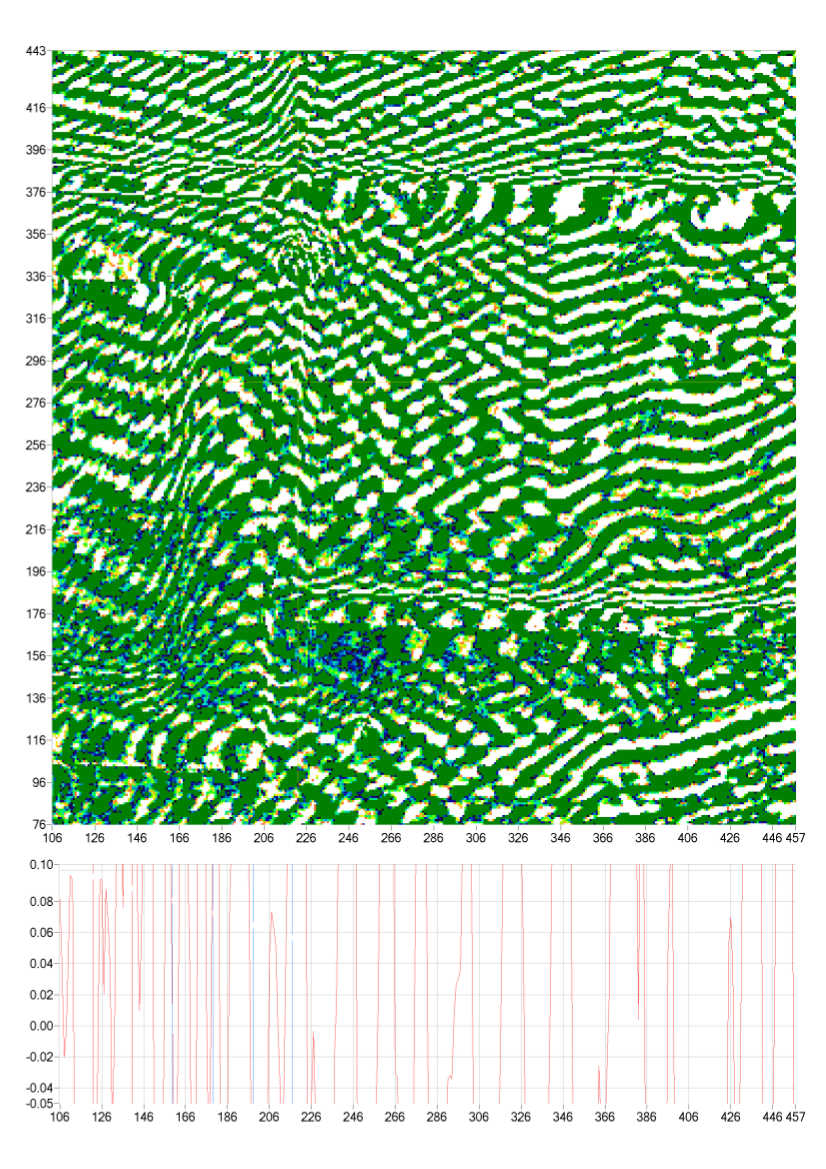
\includegraphics[width=0.3\linewidth]{figures/Normal_abs2_horiz}
\hspace{.2\linewidth}
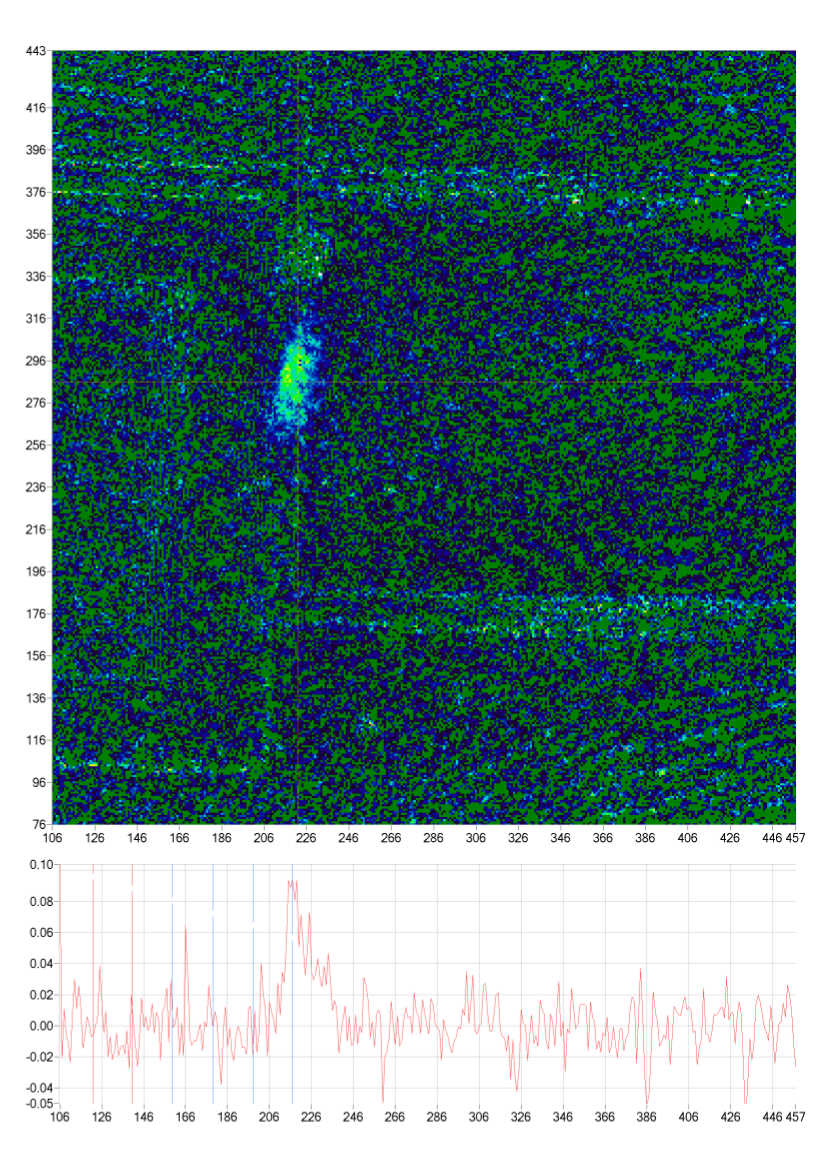
\includegraphics[width=0.3\linewidth]{figures/RF_abs2_horiz}
\caption[Effet de l'algorithme de réduction des franges]{
Images du nuage atomique froid par absorption du faisceau sonde face.
\`A gauche, l'image est traitée selon l'équation \eqref{eq:atomic_density}.
\`A droite, la même image après traitement par l'algorithme de réduction des franges.
Les graphes sous les images sont les profils de densité du nuage en coupe horizontale.
L'échelle de couleur est la même pour les deux images et a été optimisée pour l'image de droite.
}
\label{fig:Fringe_Reduction}
\end{figure}		

Troisièmement, il peut être intéressant, pour caractériser des nuages très denses, de ne pas calculer la densité optique $OD$ comme à l'équation \eqref{eq:Beer-Lambert_integ}, mais de s'arrêter à l'opération 
\begin{equation}
\label{eq:nolog_abs}
\frac{I_f(y,z)}{I_i(y,z)} = e^{-OD(x,y)} = e^{-\sigma .n(y,z)}.
\end{equation}
Nous appellerons cette opération \og absorption no-log \fg{}.
Si le nuage présente un profil de densité gaussien, cela permet de se concentrer sur les ailes de ce profil.
Dans le cas d'un nuage très dense optiquement, comme par exemple pour les mélasses optiques, le centre du nuage où la densité est très haute donne un signal d'absorption bruité.
L'ajustement du profil de densité est alors meilleur sur les bords du nuages.
La figure \eqref{fig:nolog_abs} montre l'image d'une mélasse optique par absorption de la sonde de côté, traitée d'après l'équation \eqref{eq:Beer-Lambert_integ} et d'après l'équation \eqref{eq:nolog_abs}.

\begin{figure}[!h]
\centering
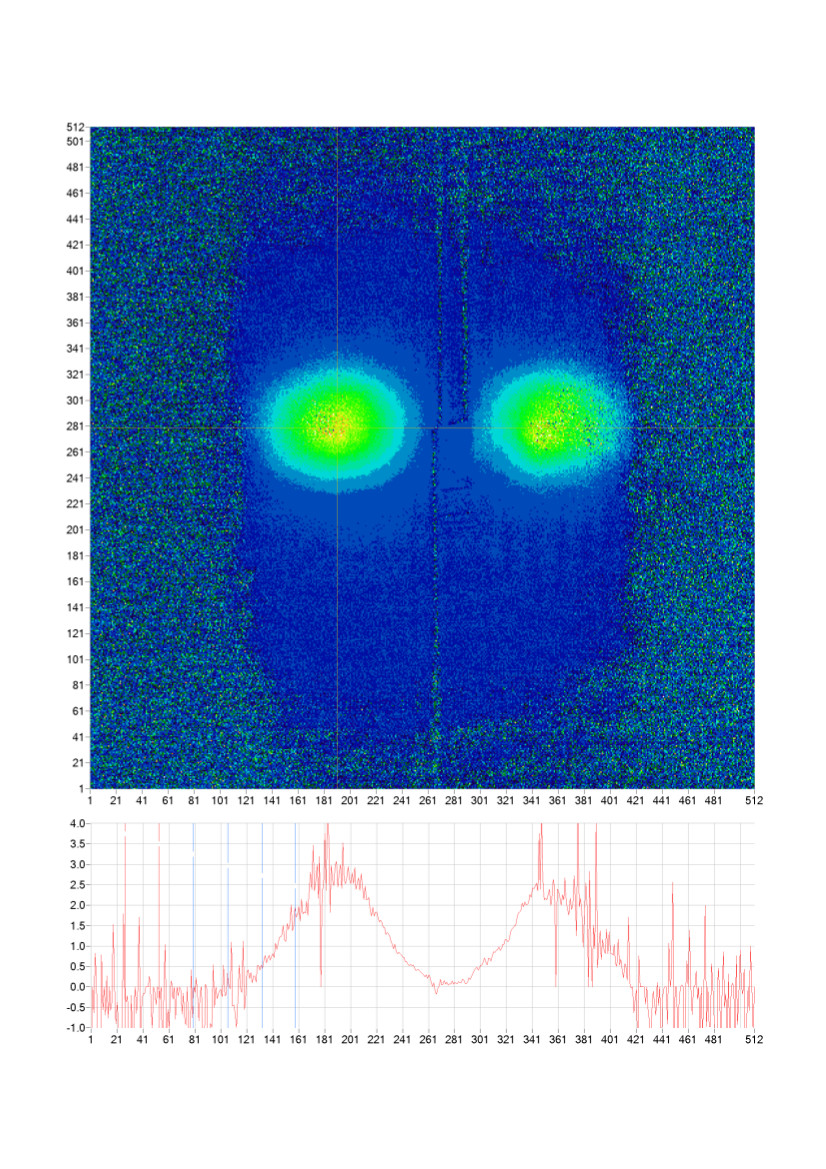
\includegraphics[width=0.4\linewidth]{figures/log_abs}
\hspace{.1\linewidth}
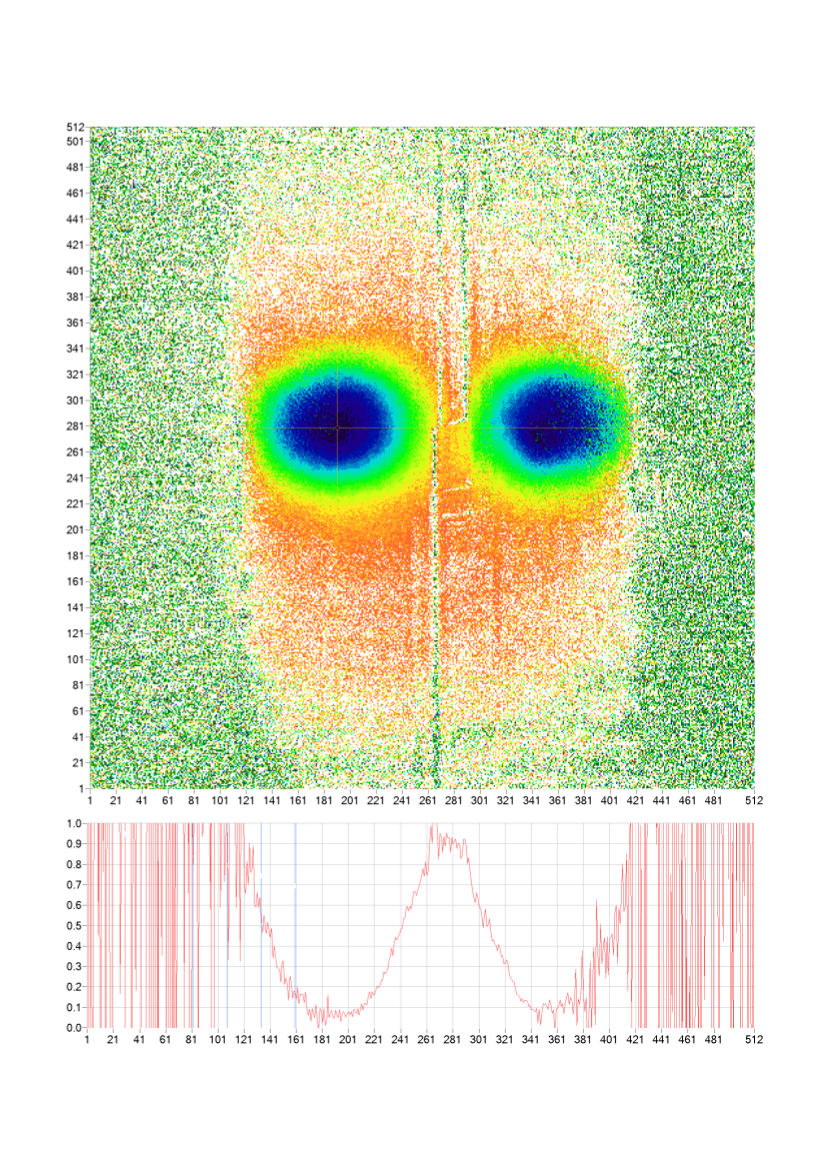
\includegraphics[width=0.4\linewidth]{figures/nolog_abs}
\caption[Absorption \og no-log \fg{} ]{
Images du nuage atomique de mélasse optique par absorption du faisceau sonde côté.
\`A gauche, l'image est traitée par absorption selon l'équation \eqref{eq:Beer-Lambert_integ}.
\`A droite, l'image est traitée selon l'équation \eqref{eq:nolog_abs}.
Les graphes sous les images sont les profils de densité du nuage en coupe horizontale.
L'échelle de couleur est différente pour les deux images, adaptée à l'échelle des profils en coupe représentés.
Les zones bruitées à gauche et à droite ne sont pas éclairées par le faisceau sonde. 
En absorption \og no-log \fg{}, le bruit est plus important dans les zones sombres, mais réduit au centre et sur les bords du nuage.
%Le bruit y est beaucoup plus important si l'on ne prend pas le logarithme du signal (image de droite).
%Cependant, le bruit y est fortement réduit au centre du nuage.
}
\label{fig:nolog_abs}
\end{figure}	

	\subsubsection*{Estimation de la température}
\noindent L'imagerie par absorption permet facilement d'estimer la température du nuage atomique.
En effet, la répartition des impulsions dans le nuage suit la distribution de Maxwell-Boltzmann tant que celui-ci n'est pas condensé.
L'évolution de la taille gaussienne du nuage après extinction du piège, dictée par l'impulsion moyenne dans le nuage,  nous renseigne alors sur sa température par l'équation de diffusion :
\begin{equation}
\label{eq:tempfit}
\Delta^2 x (t) = \Delta^2 x(t_0) + \frac{\kb T}{m}.(t-t_0)^2,
\end{equation}
où $\Delta x$ est l'extension spatiale du nuage dans la direction $x$, $t$ le temps et $t_0$ la référence de temps, $\kb$ la constante de Boltzmann, $m$ la masse d'un atome et $T$ la température du nuage.
En imageant le nuage à différents moments de son expansion (\og temps de vol \fg{}) et en ajustant la largeur gaussienne du profil à l'équation \eqref{eq:tempfit}, on accède à la fois à la température $T$ du nuage et à sa taille initiale dans le piège $\Delta x(t=0)$.
		
	\subsection{Quelques nuages typiques}
\noindent Nous avons décrit ici les éléments de notre dispositif qui servent à produire et caractériser des nuages d'atomes ultra-froids.
Le tableau \ref{tab:nuages} présente les caractéristiques principales des différents types de nuages atomiques que nous utiliserons pour y exciter des atomes de Rydberg.

\begin{table}[h!]
	\centering
	\caption[Quelques nuages typiques]{Quelques nuages typiques de notre expérience.
	Pour chacun, nous donnons les caractéristiques suivantes : nombre d'atomes $N$, taille $Delta x$ du nuage selon $x$, taille $\Delta y,z$ du nuage selon $y$ et $z$, température $T$ est distance à la puce $d$.
	}
	\label{tab:nuages}
	\begin{tabular}{c | c c c c c}
		\toprule\midrule
		{nuage}
		&N 
		&$\Delta x$
		&$\Delta y,z$
		&T
		&d
		\\
		\midrule
		QUAD-MOT
		&quelques \num{e8}
		&
		&
		&\SI{400}{\uK}
		&\SIrange{1}{3}{\mm}
		\\
%		U-MOT lointain
%		&
%		&
%		&
%		&idem
%		&idem
%		\\
		U-MOT proche
		&\SI{e7}
		&\SI{200}{\um}
		&\SI{200}{\um}
		&\SI{40}{\uK}
		&\SI{600}{\um}
		\\
		mélasse optique
		&\SI{5e6}
		&\SI{80}{\um}
		&\SI{80}{\um}
		&\SI{10}{\uK}
		&\SI{600}{\um}
		\\
		piège mag. chaud
		&\SI{1.5e6}
		&
		&
		&\SI{40}{\uK}
		&
		\\
		piège mag. froid
		&\SI{1.2e4}
		&\SI{45}{\um}
		&\SI{4.5}{\um}
		&\SI{0.75}{\uK}
		&\SI{450}{\um}
		\\
		BEC
		&\SIrange{8000}{20000}
		&
		&
		&\SIrange{30}{80}{\nano\K}
		&
		\\
		\midrule
		\bottomrule
 	\end{tabular}
\end{table}

\noindent Ces différents nuages d'atomes froids, ou ultra-froids, vont nous permettre d'explorer l'excitation d'atomes de Rydberg dans différentes conditions.